\documentclass{UoYCSproject}
\usepackage{color,soul}
\usepackage{graphicx}
\usepackage{amsmath}
\usepackage{textgreek}
\usepackage{amssymb}

\addbibresource{refs.bib}

\author{Patrick Buhagiar}
\title{The Impact of Macroeconomic Parameters and Global Markets on Forecasting the FTSE Index}
\date{2018-September-11}
\supervisor{Dimitar Kazakov}
\MIP
\wordcount{11404}

\includes{Appendices \ref{cha:usefulpackages}, \ref{cha:gotchas} and
  \ref{cha:deptfac}}

\excludes{\autoref{cha:quoteex}}

\abstract{ 
     Financial forecasting is increasingly becoming a popular area of interest in machine learning, mainly due to the high benefits that it offers through several commercial applications \cite{majhi2007stock}. Choosing the right data is a crucial step to building the right predictive model. This study attempts to measure the impact of incorporating macroeconomic data and closing prices from global stock markets when forecasting the direction of the FTSE stock market index. The analysis of the results show that while global stocks markets greatly influence the predictive perform of a model, macroeconomic data did not achieve any significant improvement to predicting the direction of the index. 
     
}

\acknowledgements{A special thanks goes to my supervisor, Dimitar Kazakov, for his guidance throughout this study. This work would not have been possible without the continuous support of my family and friends, who have always been there for me through thick and thin.}
\bibliography{refs}
\begin{document}

\maketitle

\listoffigures
\listoftables

\label{sec:start}
\thispagestyle{empty}\cleardoublepage

\chapter{Introduction}
\label{cha:Introduction}
For millennia, people have yearned for the ability to predict the future. while this ability has remained elusive, it is possible, now more than ever, to make an informed estimate thanks to the recent advancements in machine learning. Research keeps pushing the boundaries of machine learning everyday, from discovering new methods and architectures, to building more efficient and dedicated hardware that help expand existing capabilities. The main driver behind this push is not just academia, but also the industry.  Financial forecasting is one example where the industry is heavily investing in, as it offers high benefits through many commercial applications \cite{majhi2007stock}.

Financial forecasting is the ability to predict the outcome of companies, markets or economies. For entities such as investment firms, knowing what the future holds can be useful because it allows them to make smart investments, and thus maximise profits. An essential aspect to financial forecasting is choosing the most influential data \cite{zhong2017forecasting}. With regards to stock market prediction, literature has provided several methods and architectures that combine different external data sets to predict stock market indices, such as economic data, fundamental analysis, exchange rates, and even calendar based events such as earning announcements. This study will add further to this pool of research by measuring the impact of incorporating macroeconomic and global stock market data when predicting the direction of the FTSE stock market index.   

The following chapters are organised as follows. Chapter \ref{cha:literaturereview}, Literature Review, will explain the underlying economic, financial theory and machine learning concepts, while discussing different approaches for financial forecasting. Chapter \ref{cha:problemanalysis}, Problem Analysis, compares and contrast the different approaches to stock market prediction, and clearly defines the objectives, requirements, and chosen approach for experimentation in this study. Chapter \ref{cha:implementation}, Design and Implementation, further describes in detail the design choices and methodology for achieving the objectives mentioned in Chapter \ref{cha:problemanalysis}. The results of this study are shown and discussed in Chapter \ref{cha:resultsandevaluation}, and finally Chapter \ref{cha:conclusions} closes off with some final remarks and potential future work. 

\chapter{Literature Review}
\label{cha:literaturereview}

\section{Macro and Micro Economics}
\label{macroandmicro}
According to Adam Smith, the father of modern economics, the economy is a mix of micro and macro economics where every entity has individual interest towards gain, such that this gain is also linked to the overall benefit of the market as a whole \cite{smith1950inquiry}. Macroeconomics is the study of the behaviour, performance and trends of an economy as a whole. Macro-economists evaluate a variety of economy-wide phenomena such as inflation, gross domestic product (GDP) and unemployment. To keep the economy in check, governments look at these factors to aid them in economic policy decision making. Microeconomics on the other hand is the study of how individuals make economic decisions and their effect on the economy. These individuals are classified as consumers, producers and resource owners \cite{dwivedi2002microeconomics}. These individuals interact with the supply and demand for resources while using indicators, such as interest rates and money, as a pricing mechanism. 

Despite being split into two different studies, macroeconomics and microeconomics are deeply interlinked with each other since they contain overlapping issues. They can be considered as opposite approaches, where macroeconomics take a top-down approach and microeconomics a bottom-up approach to analysing an economy. As an example of how these two studies complement each other, it is evident that a stock market's long-term performance is heavily coupled with the economy's performance \cite{davis2008macroeconomic}. This coupled relationship can be seen in Figure \ref{fig:gdpvssp500} which shows a normalised plot for the U.S. GDP and the S\&P 500 index. In this case, it comes to no surprise that investment analysts focus on economic performance expectations to determine the future prospects of stock markets.

\begin{figure}[h]
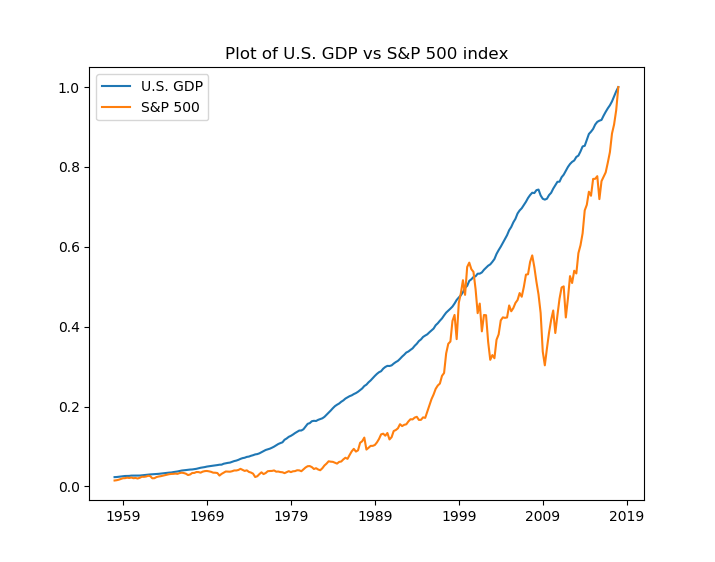
\includegraphics[width=10cm]{GDPvsSP500}
\centering
\caption{Normalised quarterly data from 1958 to 2018 for U.S. GDP and S\&P 500 index. Sources: Standard \& Poor's, U.S. Census Bureau} 
\label{fig:gdpvssp500}
\end{figure}

\subsection{Inflation}
Inflation is the rate at which the general level of prices for goods and services is rising \cite{inflation}. As a result of inflation, the purchasing power of a currency decreases. If the price of milk costs \pounds $1$ this year, then with an inflation rate of $2$\% it will cost \pounds $1.02$ the following year. Deflation is the opposite of inflation, where the general level of prices decreases. Central banks measure this inflation rate and try to limit inflation, while avoiding deflation, so as to keep the economy running smoothly. While high inflation should be avoided, deflation is much more catastrophic and has helped cause the worst economic meltdowns in U.S. history \cite{fleckenstein2013deflation}. If there is deflation, people refrain from consuming goods because they know that prices will be cheaper in the future. This will drastically reduce the demand for goods which will cut corporate profits, lower wages and reduce the work force, hence resulting in a weaker economy. For an economy to function well, both the consumers and producers must be willing to consume and produce. 

\subsection{Balance of Trade}
The balance of trade is the difference between the value of a country's imports and exports during a certain period \cite{balanceoftrade}. Economists sometimes refer to the balance of trade to measure the relative strength of a country's economy. The balance of trade can be calculated with the following simple formula:

\begin{equation}
    Balance Of Trade = Imports - Exports
\end{equation}

A country that imports more than it exports is described as having a trade deficit, otherwise it would have a trade surplus. If a country that has a trade deficit does not balance out with a high level of service exports, then it would have to borrow money. Borrowing money could lead to the value of the country's currency to fall, thus resulting in consumers paying more for foreign imports \cite{2003economics}. Alternatively, a country that has a trade surplus lends money to deficit countries. As of 2016, China has the highest trade surplus in the world, with a surplus of \$$510$ Billion \cite{tradesurplus}.   

\subsection{GDP}
Historically, the gross domestic product (GDP) is one of the most important variables when it comes to measuring the health of an economy. A country's GDP is the total value of all final goods and services produced in the economy \cite{2003economics}. GDP helps define the size of an economy. The bigger the GDP, the more goods and services are being produced, thus the healthier the economy.  There are many factors that affect the GDP such as productivity, labour force size, life expectancy, higher initial schooling, lower inflation and lower fertility \cite{barro1996determinants}. 

\subsection{Unemployment Rate}
The unemployment rate is the percentage of the labour force that is jobless \cite{unemployment}. In a weak economy, jobs tend to be scarce, hence the unemployment rate would be expected to rise. Alternatively, a healthy economy is more likely to have more jobs available, thus the unemployment rate would decrease. This means that the unemployment rate is another factor that highly affects a country's GDP \cite{bean1993unemployment}. A low unemployment rate means that more people are employed and getting paid, which brings in more money into the economy, ergo increase GDP.  

\subsection{Interest Rate}
An interest rate is a percentage of the amount that one pays when borrowing or gets paid when saving money \cite{interestrate}. If \pounds $1000$ is placed into a savings account with a $1$\% interest rate, there will be \pounds $1010$ the following year.  The bank rate is the most important interest rate in an economy and is set by the central bank. The bank rate, also known as base rate, is the rate of interest payed on reserve balances held by commercial banks. Increasing the bank rate makes borrowing more expensive which means people will spend less in order to pay off their debts or benefit more from saving. In this scenario, inflation will decrease. Ultimately, interest rates can be considered as a tool for monetary policy that can be used to contain inflation within an expected range \cite{christiano1999monetary}. 

\section{Financial Markets}
\label{financialmarkets}
A financial market is a marketplace for buying and selling securities such as stocks, bonds and currencies \cite{financialmarket}. Trading occurs on what is called an exchange. In the case of stocks, this is called a stock exchange and can either be in a physical location (like NYSE) or an electronic system (like NASDAQ). Companies that are traded on an exchange are referred to as a listed company. Otherwise, securities that are not listed are sold Over-The-Counter (OTC). Companies that trade shares OTC are typically riskier companies that did not meet the requirements to be listed on the stock exchange \cite{stockexchange}. As of June 2017, the stock exchange with the highest market capitalisation is the New York Stock Exchange (NYSE) at \$$21$ trillion \cite{nyse}. 
These stock exchanges do not operate 24 hours a day and are closed throughout the weekend and bank holidays. Table \ref{tab:markets} lists the opening and closing times of some stock exchanges around the world. 

\begin{table}[h]
    \centering
    \begin{tabular}{|c|c|c|} \hline
        \textbf{Stock Exchange} & \textbf{Open (UTC)} & \textbf{Close (UTC)} \\ \hline
        London & 08:00 & 16:30 \\
        New York & 14:30 & 21:00 \\
        Paris & 08:00 & 16:30 \\
        Frankfurt & 07:00 & 19:00 \\
        Hong Kong & 01:30 & 08:00 \\
        Tokyo & 00:00 & 06:00 \\
        \hline
    \end{tabular}
    \caption{Opening and closing times of stock exchanges.}
    \label{tab:markets}
\end{table}

\subsection{Stock Market Index}
Another way to measure the value of a stock market, other than the total market capitalisation, is to refer to what is called a stock market index. A stock market index is computed from the prices or market capitalisation of a few selected stocks, typically from the largest and most influential companies in that market. The Dow Jones Industrial Average (DJIA) is one of the oldest, most well-known stock market index in the world, which takes the stock prices of 30 companies in the United States across different industries, such as Apple, American Express, Coca-Cola and ExxonMobil. Experts however feel that the DJIA is \textit{"no longer a great reflection of the market [since] it only covers 30 stocks [and] puts too much emphasis on the price rather than a market's capitalisation"} \cite{dowproblem}. For the United States, a better alternative is the S\&P 500, which is much more diverse than DJIA because it includes $500$ companies and uses a market capitalisation-weighted index. The main goal of these stock market indices is to represent a broad economy. Table \ref{tab:indices} lists a few of the most popular stock indices, along with the region and the number of companies they represent. 

\begin{table}[h]
    \centering
    \begin{tabular}{|c|c|c|c|} \hline
        \textbf{Index} & \textbf{Trading Symbol} & \textbf{Region} & \textbf{Index Size} \\ \hline
        S\&P 500 & GSPC & U.S.A & 500 \\
        FTSE 100 & UKX & U.K. & 100 \\
        DAX & GDAXI & Germany & 30 \\
        CAC 40 & FCHI & France & 40 \\
        EURO STOXX 50 & SX5E & Eurozone & 50 \\
        NIKKEI 225 & NI225 & Japan & 225 \\
        HANG SENG & HSI & Hong Kong & 50 \\
        \hline
    \end{tabular}
    \caption{Table of popular stock market indices.}
    \label{tab:indices}
\end{table}

\subsection{Market Contagion}
One of the major shifts in the last few decades is globalisation, which consequently has increased openness and interpenetration of national economies and sovereign states \cite{scott1999regions}. As a result, regional markets have started to be more correlated with each other. Market contagion refers to this correlation, where market changes or disturbances spread from one regional market to another. This means that a financial crisis in one region will create a domino effect and weaken other economies. A good example of this is the \textit{Great Depression} in the 1930s, which originated in the United States, and resulted in the global GDP falling by $15$\% in the first $3$ years \cite{rogerhistoryrepeating}. A more recent example is the financial crisis of 2008, the effects of which still linger on in some countries \cite{2008crisis}.  

Market contagion can easily be visualised and quantified. Figure \ref{fig:stockindexplot} contains a scaled plot of the indices in Table \ref{tab:indices} over a $5$ year period. From observing the structure of the indices, it is evident that markets are connected globally, where markets seem to fall and rise together. The scatter matrix plot in Figure \ref{fig:scatterplot} further emphasises the correlation between global markets. As this study will be predicting the direction of the FTSE index, we can see that FTSE has a strong correlation with CAC, DAX and STOXX, all of which are European markets. There is also good correlation with the S\&P 500, and less correlation with HKSE and NIKKEI. Table \ref{tab:correlations} quantifies the correlations between the FTSE stock market index and the other stock market indices mentioned in Table \ref{tab:indices}. 

\begin{figure}[h]
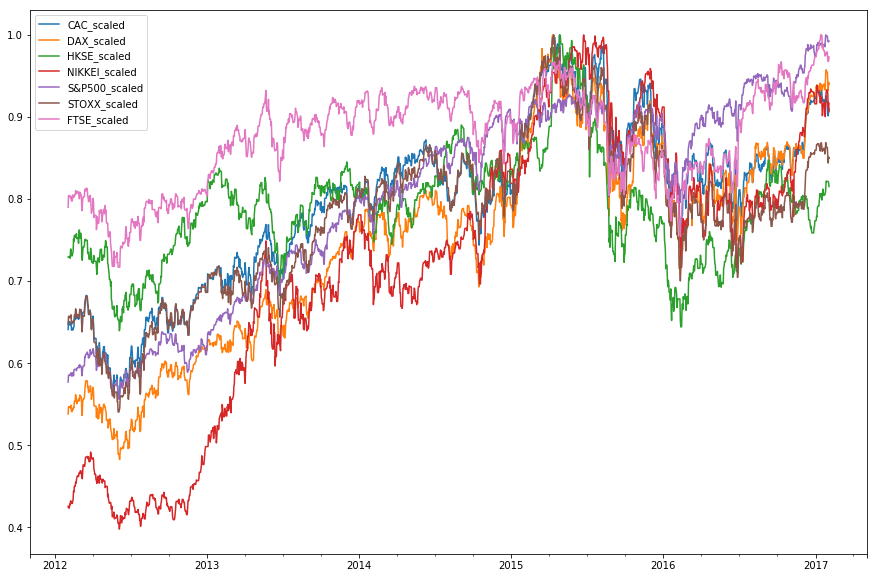
\includegraphics[width=12cm]{scaled_plot_of_indices}
\centering
\caption{A scaled plot of the CAC, DAX, HKSE, NIKKEI, S\&P 500, STOXX and FTSE stock market Indices} 
\label{fig:stockindexplot}
\end{figure}


\begin{figure}[h]
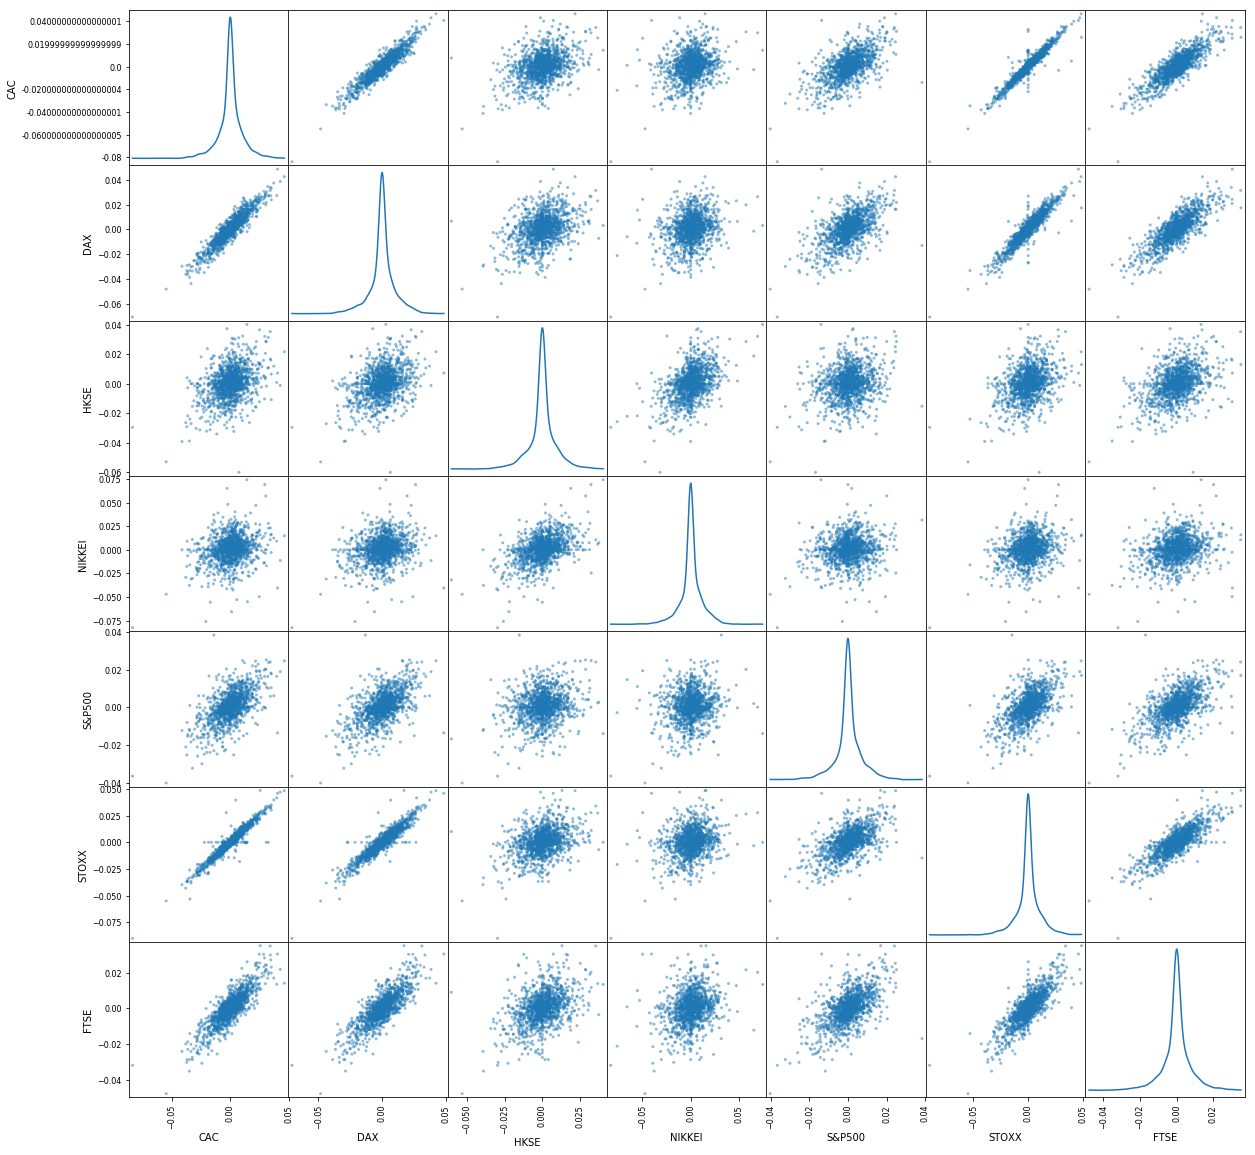
\includegraphics[width=12cm]{market_correlation}
\centering
\caption{A scatter matrix plot showing the correlations between each market.} 
\label{fig:scatterplot}
\end{figure}

\begin{table}[h]
    \centering
    \begin{tabular}{|c|c|} \hline
        \textbf{Stock Matket Index} & \textbf{Correlation} \\ \hline
        CAC &       0.848935 \\
        DAX  &     0.817487\\
        STOXX &    0.818773\\
        HKSE   &   0.417783\\
        NIKKEI  &  0.268837\\
        S\&P 500   & 0.587923\\

        \hline
    \end{tabular}
    \caption{The correlation between the FTSE stock market index and other stock market indices.}
    \label{tab:correlations}
\end{table}


\subsection{Market Hypotheses}
The following subsections give a quick overview for some of the well known market hypotheses. A more detailed discussion can be found in Matthew Butler's work \cite{butler2012computational}.
\subsubsection{Efficient Market Hypothesis}
The Efficient Market Hypothesis (EMH) was introduced by Fama in 1970  \cite{malkiel1970efficient} and is frequently cited in the field of finance and economics. It states that a market is said to be efficient if the stock price of a company, at any given time, truly reflects the value of that company. This means that there is no point in studying past stock prices in search for patterns to predict future prices. While many academics refer to a large body of evidence in support of EMH, an equal amount of evidence also contradicts it. Jensen's \cite{jensen1978some} paper finds that as better data becomes available, more inconsistencies with EMH emerge. It concludes that there are flaws with EMH and over time we will better understand these flaws and thus gain a better understanding of the markets. Another paper by Malkiel \cite{malkiel2003efficient} points out that while evidence has proved EMH to be useful in the past, certain conditions have deemed EMH inefficient for the current modern economy. Nonetheless, economists have not yet reached a consensus about whether financial markets are indeed efficient \cite{lo2004adaptive}.  

\subsubsection{Adaptive Market Hypothesis}
AMH is an improved version of EMH introduced by Andrew Lo \cite{lo2004adaptive}. He explains that emerging studies have challenged EMH, arguing that markets are actually driven by fear and greed rather than being rational. AMH seeks to add behavioural alternatives to EMH by applying the principles of evolution to financial interactions where the market is seen as an evolving entity \cite{lo2004adaptive}. These evolutionary principles are competition, adaptation and natural selection. Lo further expands on AMH in another paper \cite{lo2005reconciling}
by delving into a neuroscience perspective.

\subsubsection{Random Walk Hypothesis}
Another theory consistent with EMH is the random walk hypothesis. It states that stock prices cannot be predicted because they are random in nature. It was introduced in Burton Malkiel's book "\textit{A Random Walk Down Wall Street}" \cite{malkiel1973random}. Similar to EMH, it also suggests that there is no point in exploiting patterns in historical data to gain profits.  

\subsubsection{Chaos Theory}
Chaos theory is a mathematical concept that deals with nonlinear models, essentially anything which is effectively impossible to predict or control, such as weather, brain states or, in this case, stock markets. In chaos theory, price changes can be determined through mathematical equations predicting factors such as a trader's own personal motives, volume changes, acceleration of the changes, and the momentum behind the changes \cite{chaostheory}. Chaos theory however is highly dependent on the initial conditions set, and produces very diverging outputs with the slightest change in inputs \cite{kellert1993wake}. 

\section{Financial Analysis Techniques}
\subsection{Technical Analysis}
Technical analysis assumes that history tends to repeat itself, thus analysing past patterns can be used for predictive purposes \cite{levy1966conceptual}. For financial markets, this means looking at past stock prices for predictions rather than its components. Technical analysis is based on three major assumptions:
\begin{enumerate}
    \item The stock price is reflective of the entire company's influential factors.
    \item Stock price movements follow trends.
    \item History repeats itself in terms of price movements.
\end{enumerate}

\subsection{Fundamental Analysis}
Fundamental analysis takes a wider approach than technical analysis by studying the past and present market data, as well as economic-level, industry-level and company-level indicators such as earnings, risk, growth and competitive position. Papers such as that of Lev and Thiagarajan \cite{lev1993fundamental} attempt to identify which fundamentals or financial variables, over a certain period of time, were suitable for performing financial forecasting. These fundamentals can either be quantitative or qualitative. Quantitative fundamentals are numeric values such as revenue and profit, while qualitative fundamentals are those that are based on the character or quality of a variable, such as brand recognition and competitive position. 

Unlike technical analysis, fundamental analysis assumes that the stock market is not fully representative of the actual value of the stock. Fundamentalists however do believe that the market will reflect these fundamentals in the long run, thus encouraging investors to find opportunities to buy stocks at a reduced price by estimating the actual value of the stock. 

\subsection{Time Series Analysis}
A time series is a collection of numerical data points collected at constant time in the form of a sequence. With time series analysis, one can obtain meaningful statistics and other characteristics of data, such that one can understand the data and build a model based on the given patterns. Extracting such models will allow one to forecast future values. 

Two key properties of time series are that they are time dependent, and that most of them have some form of seasonality trends. Seasonality trends mean that the time series consists of variations specific to a particular time frame. Due to these properties, forecasting time series requires the data to be stationary. A time series is said to be stationary if both the mean and autocovariances do not depend on the date \cite{hamilton1994time}. 

\subsubsection{Making a Series Stationary}
\label{subsec:stationary}
Making a time series stationary involves removing trends and seasonal changes. There are several methods for making a time series stationary, some of which can be combined together:
\begin{enumerate}
    \item \textbf{Transformation:} Trend can be reduced by transforming the data. this can be anything from calculating the log, square-root, cube root etc.  
    \item \textbf{Moving Average:} This method takes the average of \textit{k} consecutive values, depending on the frequency of the time series, for example 12 months, or 1 year. This is also called a \textit{rolling mean}. 
    \item \textbf{Differencing:} This technique involves subtracting each value with it's previous value.
    \item \textbf{Decomposition:} This approach consists of modelling trend and seasonality separately, and returning the remaining part, typically referred to as \textit{residual}. 
\end{enumerate}

\subsubsection{How to Test for Stationarity}
\label{subsec:testingstationarity}
Statistical tests can be utilised to examine the stationary assumptions by decomposing the time series into three elements: trend, random walk, and stationary error. Two popular tests are the Kwiatkowski-Phillips-Schmidt-Shin (KPSS) test and the Augmented Dickey-Fuller (ADF) test.

The ADF test was introduced in 1979 by David Dickey and Wayne Filler \cite{dickey1979distribution}. This test determines whether an autoregressive model contains a unit root, which is a feature that determines how strongly a time series is defined by a trend.

The KPSS method proposes a similar test to the ADF method, however while the ADF test's null hypothesis is the presence of a unit root, the null hypothesis for KPSS is the opposite. 

\section{Machine Learning}
Machine learning is a field of science concerned with building models capable of making predictions used to classify data, improve in performance and expand their knowledge through experience, without any human intervention \cite{mitchell1997}. 
In general, machine learning can be divided into into the following disciplines:

\begin{enumerate}
    \item \textbf{Supervised Learning:} These algorithms are trained using labelled training example inputs by generalising and constructing a learning model based on patterns found within the data. This generalised model can then be used to make predictions on unforeseen data. Predictions can either be classification (discrete outputs) or regression (continuous outputs). 
    
    \item \textbf{Unsupervised Learning:} Unlike supervised learning, there is no training set in unsupervised learning. Instead, the algorithm must make sense of unlabelled data on its own, such as automatic clustering.
    
    \item \textbf{Semi-supervised Learning:} This is similar to supervised learning, however the algorithm uses both labelled and unlabelled data for training. This is useful when it is too expensive to construct a fully labelled training set. 
    
    \item \textbf{Reinforcement learning:} These algorithms learn through trial and error which actions yield the greatest rewards. It is typically used for robotics, self driving cars and gaming.  
\end{enumerate}

\subsection{Artificial Neural Networks}
An artificial neural network (ANN) attempts to model the information processing capabilities of nervous systems \cite{rojas2013neural}. It can be seen as a web of neurons and synapses (links between neurons), capable of performing computations on a given input by learning and identifying patterns. The fundamental unit of an ANN is the Perceptron, also known as an artificial neuron, which is an abstraction of a biological neuron. One can identify the similarities between an artificial neuron and a biological neuron in Figures \ref{fig:artificialneuron} and \ref{fig:biologicalneuron}.  

\begin{figure}[h]
\includegraphics[width=10cm]{perceptron.png}
\centering
\caption{An artificial neuron (Perceptron).} 
\label{fig:artificialneuron}
\end{figure}

\begin{figure}[h]
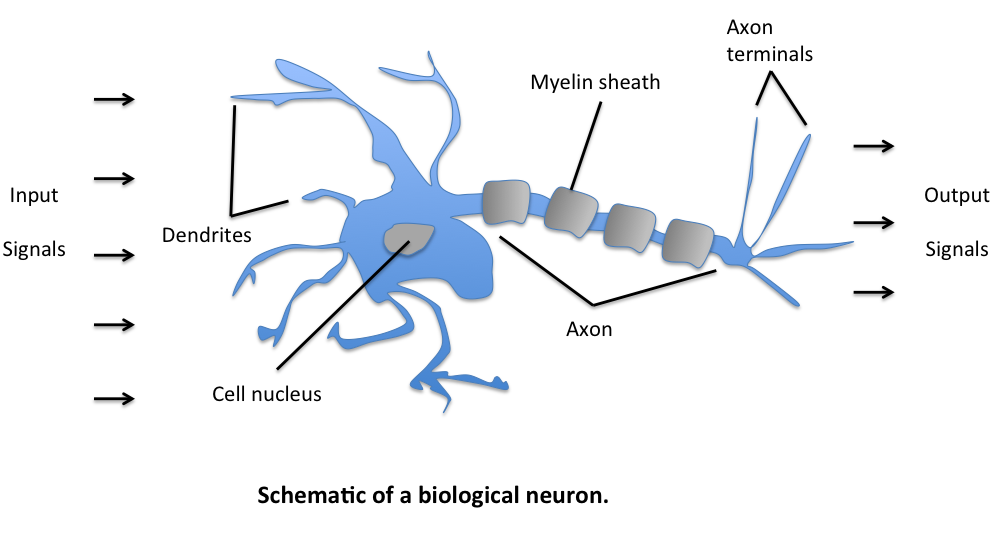
\includegraphics[width=10cm]{perceptron_neuron.png}
\centering
\caption{A biological neuron \cite{neuron}.} 
\label{fig:biologicalneuron}
\end{figure}

The artificial neuron has four main components: inputs $x$, weights $w$, the activation function $f(x)$ and the output. The inputs are the features or attributes, also known as feature vector, which is simply represented as an n-dimensional vector consisting of binary or numerical values. These inputs are the equivalent of the input signals being received by the dendrites in Figure \ref{fig:biologicalneuron}. These inputs are then multiplied by weights and fed into an activation function. The output is the result of this activation function. In its simplest form, the output of an activation function is binary, which in the biological neuron translates to whether the neuron is firing an electrical signal or not. There are many types of activation functions, however the popular ones are the sigmoid function, $tanh$ function, and the softmax function. If an activation function does not output a discrete value, then a threshold is set, for example:  \[ f(x) =
  \begin{cases}
    1       & \quad \text{if } x \geq 0\\
    0       & \quad \text{if } x < 0
  \end{cases}
\]
Training a model involves determining the right weight values that causes the artificial neuron to output the correct result. This is done using gradient descent on the training set. 

\begin{figure}[h]
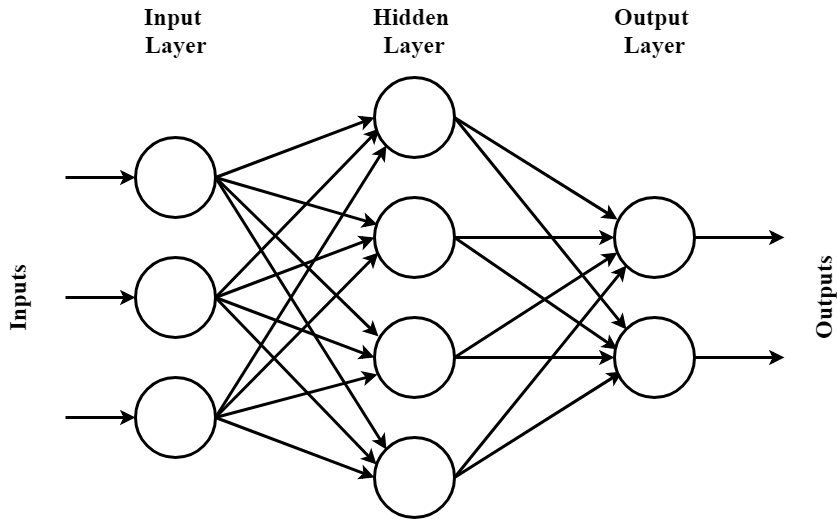
\includegraphics[width=10cm]{feedforward.png}
\centering
\caption{A feed forward network.} 
\label{fig:feedforward}
\end{figure}

\subsection{Feed Forward Neural Network}
A feed forward neural network is an architecture that consists of layers of neurons, where the output of one neuron can be fed into another neuron, without any loops \cite{jain1996artificial}. Therefore, all information that is fed into the input layer flows through the hidden layers until it reaches the output layers, such that the outputs of each layer only affects the next layer, without any feedback \cite{jhaartificial}. An example of a feed forward network can be seen in Figure \ref{fig:feedforward}, which contains an input layer, one hidden layer, and an output layer. If a feed forward network has more than one hidden layer, then it is referred to as a deep architecture. 

Some of the architectural decisions that must be taken with feed forward networks include deciding on how many hidden layers and nodes should be included in the network. Cybenko \cite{cybenko1989approximation} introduced the first version of the universal approximation theorem which states that a feed-forward network with one hidden layer, a certain number of nodes and the appropriate parameters is capable of learning the majority of problem cases. Hornik \cite{hornik1991approximation} further expands on this theorem and shows that it is not the choice of activation function, but rather the choice of feed forward architecture that brings out the full potential of being universal approximators. Given this theorem, one might wonder why anyone would need a deep architecture. While this theorem holds for \textit{representing} a wide array of problems, it does not deal with the algorithmic \textit{learnability} of parameters. It was always possible to build deep networks with feed forward networks. They were just not particularly good at training them before Hinton et al. \cite{hinton2006fast} showed how a many-layered feed forward neural network can be effectively trained one layer at a time. 

\section{Financial Forecasting}
Stock market forecasting is one of the most challenging areas of research lately due to stock markets being "\textit{essentially dynamic, non-linear, complicated, non-parametric and chaotic in nature}" \cite{tan2005brain}. Additionally, stock market movements are influenced by several macroeconomic factors such as political events, economic conditions, movement of other stock markets and investor expectations \cite{zhang2009stock}. Despite these challenges, predicting stock markets is a very attractive problem to solve thanks to the high benefits that it can offer through many commercial applications \cite{majhi2007stock}. 

The difficulty of stock market prediction has raised questions on whether this is achievable. The EMH and the Random-Walk Hypothesis both claim that there is no value to predicting a market price since the current price truly reflects the value of the stock. However, researchers believe that markets are actually inefficient since market participants are unable to respond immediately to newly released information \cite{jensen1978some}. 

The recent trend is to develop models for forecasting financial data \cite{majhi2007stock}. Forecasting models can either be statistical or soft-computing models. The most popular statistical forecasting model is the Auto-regressive Integrated Moving Average (ARIMA) model. It predicts future values of a series based on its own inertia and is suitable for short-term forecasting with data that contains stable or consistent patterns. ARIMA however is a linear non-stationary model, therefore other alternatives must be considered for forecasting non-linear series, such as stocks \cite{wang1996stock}. 

\subsection{Soft Computing Techniques}
Unlike statistical models, AI models such as ANNs, fuzzy systems, and genetic algorithms are driven by multivariate data with no required assumptions, and thus have been applied to forecast financial variables on several occasions \cite{zhong2017forecasting}. 

\subsubsection{Equation Discovery}
Equation discovery is a machine learning approach for learning quantitative laws and models from measured numeric data, expressed in the form of equations \cite{Todorovski2010}. Equation discovery can also be used for financial forecasting.  \cite{kazakov2008equation}  used LAGRAMGE, an equation discovery tool, for modelling macroeconomic variables. There are an infinite amount of equations that can be found when trying to model a situation. To help restrict the search space, LAGRAMGE makes use of user defined context free grammars. Georgiev and Kazakov in \cite{Georgiev2012Equation} used LAGRAMGE to search for ordinary differential equation models for macroeconomic data. They conclude that differential equations match ordinary ones with regards to accuracy, while having a better forecast range \cite{Kokov2012Equation}.  

\subsubsection{Artificial Neural Networks}
One popular technique for financial forecasting is to use ANN based models, which are capable of approximating any nonlinear function to a high degree of accuracy. They are less sensitive to error term assumptions and can tolerate noise and chaotic components \cite{majhi2007stock}. ANNs have been used for stock market prediction for decades. In 1990, Kamijo and Tanigawa \cite{kamijo1990stock} used recurrent neural networks (RNN) while Ahmadi \cite{ahmadi1990testability} used back propagation (BP) neural networks to predict the stock market. Trippi et al. \cite{trippi1992trading} introduced a neural-network based intraday trading system for the S\&P 500. 

Despite being suitable for financial time series forecasting, Lawrence et al. \cite{lawrence1998noisy} point out that excessive noise in data when training BP networks could result to the network resorting to simpler, naive solutions, such as choosing the most common output. Furthermore, achieving the desirable result requires finding the right combination of network parameters, particularly learning rate, number of hidden layers and number of nodes in each layer \cite{hussain2008financial}. It has been shown that designing an ANN with the least complex architecture and the right input variables can greatly improve efficiency and accuracy \cite{atsalakis2009surveying}. Therefore, when it comes to using ANNs for financial forecasting, it is essential to choose the most influential and representative inputs which, as mentioned earlier, can be any of the various macro and micro economic factors that affect the stock market \cite{zhong2017forecasting}. 

\subsubsection{Hybrid Algorithms and Ensemble Learning}
Nowadays prediction performance is being improved by hybridising several AI techniques. Tsaih et al. \cite{tsaih1998forecasting} combined the rule-based technique and ANNs to predict daily S\&P500 direction changes on a daily basis. Zhang et al. \cite{zhang2009stock} predicted short term and long term stocks using a BP neural network incorporated with an improved bacterial chemotasix optimisation (IBCO). Asadi et. all \cite{asadi2012hybridization} proposed training a feed forward neural network with a combined of several data preprocessing techniques, genetic algorithms and the Levenberg-Marquardt (LM) algorithm. Through data transformation and input selection pre-processing methods, the resulting model yielded good prediction results and coped well with stock market fluctuations. In 2009, Ou and Wang \cite{ou2009prediction} predicted the HSI index using ten data mining techniques, such as KNN and tree-based classification, ANNs, support vector machines and linear and quadratic discriminant analysis. In 2010, Hadvandi et al. \cite{hadavandi2010developing} used a combination of genetic algorithms and feed forward neural networks to predict the TEPIX stock index.

Another recent trend in financial time series prediction is the use of ensemble learning. Ensemble learning is the combination of predictions from individually trained classifiers to form a single predictive model. Research has shown that the ensemble typically achieve better accuracy prediction, compared to the individual classifiers in the ensemble \cite{opitz1999popular}. Apart from improving the prediction performance, ensemble techniques can be used for model selection. Bagging \cite{breiman1996bagging} is one example, where classifiers train on several sub samples of the training data and then, by majority voting, the most-voted class is predicted. Another ensemble technique is random subspace, which randomly selects features from a given data set. A model is built on each subspace, and finally integrated by majority vote, similar to bagging. 

\chapter{Problem Analysis}
\label{cha:problemanalysis}
\section{Stock Market Forecasting}
The previous chapter mentioned several techniques for stock market prediction such as using statistical models, ANNs, SVM and ensemble methods. Despite having all these different approaches, the no free lunch theorem \cite{wolpert1997no} states that there is no singular model that works best for every problem. This means that while a particular approach might work for a particular problem, it might not hold for another. 

Atsalakis and Valavanis \cite{atsalakis2009surveying} provide an excellent survey on $100$ scientific articles on stock index forecasting. These articles together model $24$ stock market indices from around the world, both from well developed markets such as the U.K., U.S.A and Japan, and emerging markets such as Latvia, Singapore and Turkey. The most popular area for research is American stock indices such as S\&P 500, NASDAQ and Dow Jones.

\subsection{Inputs}
As mentioned earlier, selecting the most suitable inputs for financial forecasting is essential \cite{zhong2017forecasting}. In the aforementioned survey by Atsalakis and Valavanis \cite{atsalakis2009surveying}, the number of inputs used ranged from $2$ to $61$ variables. 

The most popular type of input for stock market prediction is stock index data, which includes opening or closing prices, as well as the daily highest and lowest values per day. This suggests that a significant amount of research prefers to use simple input data to provide predictions. \cite{barnes2000study, donaldson1999neural, halliday2004equity, tan1995conservative, pai2005hybrid, pantazopoulos1998financial} all used daily closing prices as input, while \cite{andreou2000testing, fernandez2000profitability, pan2005predicting,tang2002web} also used the closing price from previous days. 

Some studies have combined closing prices with other stock market indices, or external factors such as macroeconomic and financial variables. Examples of external factors are currency exchange rates, gold coin value, interest rates and earning announcements. \cite{ajith2003hybrid} attempts to predict the NASDAQ stock index by using closing prices from NASDAQ and seven other indices. \cite{huang2005forecasting} uses both the S\&P 500 and USD/YEN exchange rate to predict the NIKKEI stock market index. \cite{phua2001neural} forecasts the Singapore stock exchange using volume, opening, lowest, highest and closing index prices of the DJIA, NASDAQ, HIS and NIKKEI indices. \cite{siekmann1999information} used the DJIA index and the USD/EURO exchange rate to predict the DAX stock market index. \cite{tabrizi2000stock} forecasts the TEPIX stock index using the gold coin value and the USD exchange rate. \cite{levodeanschi2016} investigated the impact of using earnings calendar information in portfolio construction techniques. In general, \cite{atsalakis2009surveying} highlights that researchers tend to use a combination of exchange rates and stock index values for predicting emerging markets as they are more likely to be influenced by these factors than well established markets. Other papers that used macroeconomic and financial factors are: \cite{gradojevic2002neuro}, which used lagged interest rates and lagged order flow; \cite{thawornwong2004adaptive}, which used thirty one financial and economic variables including producer price index, industrial price index, consumer price index and money stock; and \cite{setnes1999fuzzy}, which predicted the Amsterdam stock exchange (AEX) using Dutch macroeconomic data such as money supply, long and short term interest rates, economic growth and inflation.

The majority of the articles mentioned in \cite{atsalakis2009surveying} found input data preprocessing to be useful and necessary. Sensitivity analysis is sometimes employed to help remove any redundant inputs. In several cases, input data has a wide range of values, which might reduce the effectiveness of training procedures. This can be solved by normalising the data. Alternative techniques are to use Principal Component Analysis (PCA) \cite{ajith2003hybrid}, Z-score \cite{leigh2002analysis}, and an ANFIS techniques used by \cite{atsalakis2006neuro}. 

\subsection{Forecasting Methodologies}
Neural network architectures such as feed forward and recurrent networks are the most popular forecasting architecture, amounting to 60\% of the articles surveyed in  \cite{atsalakis2009surveying}. \cite{ajith2003hybrid, andreou2000testing, pantazopoulos1998financial,phua2001neural, refenes1997neural, thawornwong2004adaptive} used feed forward neural networks while \cite{barnes2000study, leigh2002analysis, witkowska1995neural} used back propagation neural networks. Architectures typically span between one or two hidden layers, while the maximum number of input nodes used is 52. \cite{atsalakis2009surveying} comments that despite neural networks being suitable for market forecasting, difficulties tend to arise when defining the anatomy of the model, and so far the best way to determine the optimal architecture is through trial and error. 

\section{Data} 
\label{sec:data}
This study requires both macroeconomic data and stock market index data. The following subsections describe the data that was collected, while Section \ref{sec:datapreprocessing} will then explain how this data was transformed and manipulated.

\subsection{Macroeconomic Data}
This study involves predicting the direction of the UK stock market, thus it made sense to focus on collecting macro-economic data for the UK. To simplify the model, the scope of learning had been reduced to five macroeconomic variables: inflation rate, interest rate, balance of trade,  unemployment rate and GDP. These parameters were chosen because they are commonly used in literature, both for stock market prediction and modelling of macroeconomic variables. A definition for these parameters can be found in Section \ref{macroandmicro}. This data is provided by the UK Office for National Statistics which provides yearly, quarterly and monthly data for inflation and unemployment rate, yearly and quarterly data for GDP and balance of trade, and daily data for interest rate. 

\subsection{Stock Market Index Data}
This study uses historical closing prices from some of the top global financial stock market indices. Apart from FTSE, which is what will be predicted, data was collected for the following stock market indices: STOXX 50, S\&P 500, Nikkei 225, DAX 30, CAC 50 and Hang Seng. These indices were chosen precisely because they represent the most influential economies in the world, and are often used in literature for financial forecasting. Stock market indices from emerging markets are less likely to influence well established markets such as the UK.  More information about these stock market indices can be found in Table \ref{tab:indices}. All these stock market indices where collected from Yahoo Finance, except for FTSE, which was collected from \textit{www.investing.com}. 

\section{Objectives}
\label{sec:objectives}
This study seeks to measure the impact of external factors, particularly the closing prices of other stock markets and macroeconomic data, when predicting the direction of the FTSE stock market index. It does not seek to introduce a new trading tool that maximises profit, or a state-of-the-art technique for financial forecasting, but rather investigate how particular data sets can improve predictive performance. Overall, this study seeks to test the following hypotheses:

\begin{enumerate}
    \item \label{h1} \textbf{The use of closing prices from other stock market indices improves the performance for predicting the direction of a stock market index.}
    \item \label{h2} \textbf{The use of macroeconomic parameters improves the performance for predicting the direction of a stock market index.}
    \item \label{h3} \textbf{The combination of macroeconomic parameters and closing prices from other stock market indices improves the performance for predicting  the direction of a stock market index}
\end{enumerate}

For all 3 hypothesis, the null hypothesis is that the method in question makes no significant difference in prediction accuracy when compared to underlying base cases.

\section{Requirements}
\label{sec:requirements}
The requirements for this study are:

\begin{enumerate}
    \item \label{basecase} \textbf{Formulate base cases for predicting the direction of the FTSE index:} Two base cases were used. Model results were compared with these base cases to determine whether an improvement in predictive performance was achieved.  
    \begin{enumerate}
        \item \label{basecase1} \textbf{Base case 1:} This base is simply always predicting the direction of the stock market as going up. 
        \item \label{basecase2} \textbf{Base case 2:} This base case is a simple model that only uses historical prices of the FTSE index, without using closing prices from other stock indices or macroeconomic parameters. 
    \end{enumerate}
    
    \item \textbf{Formulate a model that incorporates historical FTSE closing prices with closing prices from other stock market indices for predicting the direction of the FTSE index:} This model was used to confirm whether hypothesis \ref{h1} holds.
    \item \textbf{Formulate a model that incorporates historical FTSE closing prices with macroeconomic parameters for predicting the direction of the FTSE index:} This model was used to confirm whether hypothesis \ref{h2} holds.
    \item \textbf{Formulate a model that incorporates historical FTSE closing prices with both macroeconomic parameters and closing prices from other stock market indices for predicting the direction of the FTSE index:} This model was used to confirm whether hypothesis \ref{h3} holds.
    \item \label{framework} \textbf{Develop a framework that can be used to train, predict and evaluate the performance of the above models:} More information on the performance measures and evaluation criteria will be covered in the next section. 
\end{enumerate}

\section{Performance Measures and Evaluation Criteria}
Performance measures can be classified as statistical measures or non-statistical measures \cite{atsalakis2009surveying}.

Examples of statistical measures are the root mean square error (RMSE), $R^2$, F1 score, the mean absolute error (MAE), the mean squared prediction error (MSPE), and statistical indicators such as autocorrelation, correlation coefficient, and standard deviation. 

Non-statistical performance measure are less common, and in financial forecasting are typically related with the economical side of the forecast. An example is accuracy, which is the percentage of correct predictions. Other non-statistical measures measure the profitability of the model, such as rate of return or average annual profit.

This study involves predicting the direction of the FTSE stock market index, thus making it a binary classification problem. As mentioned in the previous section, it is pertinent to understand that the aim of this study is to determine whether combining particular sets of data will improve the predictive performance of a model, and not to find the state-of-the-art approach for maximising profits. Nonetheless, prediction accuracy does not directly equate to more profit. When predicting direction of stock markets, one could achieve a high accuracy, however one incorrect prediction could be a drop large enough to wipe out any profits made in previous predictions. Thus, these findings are not intended to be used directly in complete trading strategies, despite perhaps being a stepping stone to improving trading strategies in the future. 

Since we have a binary classification problem, it does not make sense to use statistical performance measure such as RMSE, MAE and $R^2$ as they require continuous values. They would have been suitable to use if this study involved predicting a continuous value such as the closing price, or the percentage increase. The two performance measures that were used in this study were \textbf{accuracy} and \textbf{F1 score}. 

\subsection{Accuracy and F1 Score}
\label{subsec:accuracyandf1}

Both the accuracy and F1 score require counting the number of true positives, true negatives, false positives and false negatives. For this study, these terms have been defined as follows:

\begin{enumerate}
    \item \textbf{True Positives (TP)}: This is when a result correctly predicts that the index will rise (the positive condition).
    \item \textbf{True Negatives (TN)}: This is when a result correctly predicts that the index will fall (the negative condition).
    \item \textbf{False Positives (FP)}: This is when a result predicts incorrectly that the index will rise, when it actually falls.
    \item \textbf{False Negatives (FN)}: This is when a result predicts incorrectly that the index will fall, when it actually rises.
\end{enumerate}

Figure \ref{fig:tptnfpfn} helps visualise what these terms mean.

\begin{figure}[h]
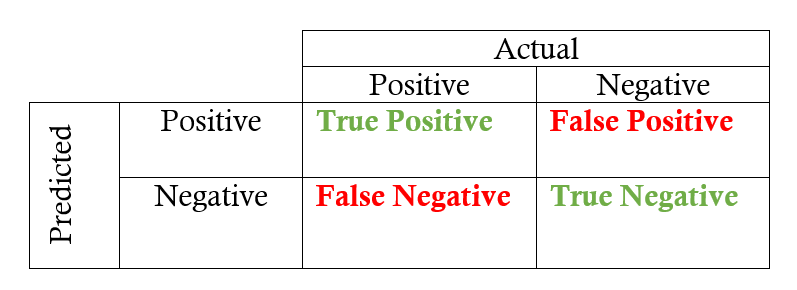
\includegraphics[width=10cm]{tptnfpfn.png}
\centering
\caption{Matrix of terminology for true and false negatives and positives \cite{precisionandrecall}.} 
\label{fig:tptnfpfn}
\end{figure}

The accuracy can be calculated with the following formula: 
\begin{equation}
\label{eq:accuracy}
accuracy=\frac{TP + TN}{TP + TN + FP + FN}
\end{equation}
This is simply the summation of correctly predicted values divided by the total number of data items.

When faced with a well balanced data set, the accuracy metric is an excellent and fair metric. There are some cases however where accuracy might not be suitable as the sole metric. As an example, imagine a model that identifies whether people at an airport are terrorists or not. This model can reach over $99$\% accuracy simply by labelling all passengers as not a terrorist, because typically there are only a handful of terrorists compared to the millions of passengers that travel in airports every year. The real performance metric in this case would be measuring how well it identifies terrorists, therefore true positives. This sort of metric is known as \textbf{recall} in statistics. Recall is the measure of the model's ability to find all relative cases (true positives) within a dataset. It can be measured by the following formula:

\begin{equation}
recall=\frac{TP}{TP + FN}
\end{equation}

Recall is also referred to as true positive rate, probability of detection or sensitivity.  

Another important statistical metric is \textbf{precision}, which measures the ability of a model to identify only the relevant data points. If we relied on just recall, then labelling all the results as positive would result in a perfect recall score of 1. Such a model would however suffer from low precision. Precision is calculated as:

\begin{equation}
precision=\frac{TP}{TP + FP}
\end{equation}

Precision is also referred to as the positive predictive value.

Depending on the problem at hand, statisticians would prefer to maximise either recall or precision at the expense of the other. As an example, in cancer screening models, one would rather maximise recall, therefore identifying patients with cancer, while accepting lower precision. However in certain cases, such as stock market prediction, a good balance of precision and recall would be appreciated, because predicting incorrectly whether a stock will increase or decrease will both have the same severe consequences: profit loss.

The F1 score can be calculated as:

\begin{equation}
\label{eq:f1}
F_1=2 \times \frac{precision \times recall}{precision + recall}
\end{equation}

In chapter \ref{cha:resultsandevaluation}, the data set that was used happened to be a well balanced data set. Therefore, accuracy was given greater priority than F1 score. The F1 score was recorded nonetheless for experiments.  

\subsection{Statistical Significance Test}
\label{sec:statisticalsignificancetest}
\subsubsection{Kruskal-Wallis Test}
The Kruskal-Wallis test is a type of non-parametric test. The term \textit{non-parametric} signifies that no assumptions are made with regards to the underlying distribution of the data, such as mean and standard deviation. Essentially, non-parametric tests can be used when the population data does not have a normal distribution. The Kruskal-Wallis test compares two or more samples, regardless of whether they are equal in size or not. The null hypothesis assumes that all samples are from identical populations.  

For this study, the test was used to determine whether all predictive models mentioned in Section \ref{sec:requirements} achieved the same accuracy (the null hypothesis), or not.  Otherwise, if it is rejected, then at least one sample originates from a different population from the others, therefore, contains a significant different in accuracy. The null hypothesis is rejected when the p-value given by the Kruskal-Wallis test is less than $0.05$.

The data sample used for this test contained a value of either one or zero, where a value of one signifies that a model correctly predicted the direction of the FTSE index, while a zero signifies otherwise.
 

\subsubsection{Wilcoxon Signed Rank Test} 
\label{sec:wilcoxon}
In the case that the Kruskal-Wallis test results in the null hypothesis being rejected, the next step would be to identify which method achieved a significant improvement in accuracy with respect to the other remaining method. This was achieved by performing the Wilcoxon signed rank test, which is another type of non-parametric test. Unlike the Kruskal-Wallis test, this test compares only two samples in order to assess whether their population mean ranks differ. The null hypothesis is that the medians of two samples are equal. The underlining assumption however is that the paired differences are independent from each other.

For this study, the test was used to determine whether two predictive models do not significantly differ from each other in terms of accuracy (the null hypothesis), or not. Each method in this study was paired with another method for this test. If the null hypothesis is accepted, then one can conclude that no significant improvement in predictive accuracy was achieved. The null hypothesis is rejected when the p-value given by the Wilcoxon signed rank test is less than 0.05.

The data sample used for this test contained a value of either one or zero, similar to the approach use for the Kruskal-Wallis test.

\section{Discussion}
\label{sec:discussion}
This chapter began by comparing and contrasting past financial forecasting techniques, primarily on what data has been modelled, how it was preprocessed, and what architectures were used. It was also shown that stock market index prediction is sometimes combined with other external data, such as economical data, to help improve prediction performance. Other works also took into consideration the closing prices of other stock market indices. However, to our knowledge, there seems to be a gap in literature where both macroeconomic data and the closing prices of other markets are used to predict a stock market index. These two types data pose some interesting questions. Globalisation has helped global markets become interrelated, resulting in market contagion. To what extent can this phenomenon be used to predict the direction of a stock market? On the other hand, macro and micro economics are deeply interlinked. If the economy is doing well, would the general mood towards stock markets be better, thus resulting in an increase in stock prices? This study aims to answer such questions, and seeks to use both sets of data in an effort to produce a better evaluation of the impact of such external factors on the direction of the FTSE stock market index.   
The next chapter will introduce both an ensemble approach and feed forward networks which will conform to the requirements in Section \ref{sec:requirements}. As previously mentioned, ensemble methods have been shown to improve prediction performance over individual classifiers in the ensemble \cite{opitz1999popular}. Both stages of the ensemble will use a feed forward artificial neural network. The ensemble approach will only be used for incorporating macroeconomic data, while simple feed forward networks will be used for the rest of the models.

The ensemble approach was inspired by the works in Matthew Butler's PhD thesis \cite{butler2012computational} where he introduced LATIS (Learning Adaptive Technical Indicator System), a forecasting algorithm that blends micro and macro modelling perspectives when applying computational intelligence techniques. LATIS consists of a meta agent that uses reputation, effectiveness threshold and return as meta parameters for choosing an action to perform. The same idea, with different parameters was applied to this study, where instead a meta agent uses macro economic parameters to select which predictive model to use. The models to be selected are several feed forward networks trained over different periods that follow the same architecture as the second base case or hypothesis \ref{h1}. This last piece is inspired by the bagging approach in ensemble learning \cite{breiman1996bagging}, where classifiers are trained on several sub sample of the training data. These sub samples are often chosen at random, however since this study deals with a time series, the order of data is crucial. An alternative option would be to take sub samples as shifted periods of data.

Stock market data is volatile in nature and fluctuates on a daily basis. Training several models over smaller different time periods instead of a single model over one large period could be beneficial because with a smaller dataset, a model would be able to better capture fluctuation patterns in greater detail. Capturing the same level of detail with the same model over a large dataset would more likely lead to overfitting. Matthew Butler also points out that \textit{"models constructed from historical information will wax and wane with the evolving market"}\cite{butler2012computational}. This suggests that predictive models lose their relevance over time, but may become good again in the future when a similar pattern in the data reappears. This can very well be applied to stock markets, especially when technical analysts assume that history tends to repeat itself in terms of price movements.

The decision for using feed forward networks was due to their popularity as a choice of architecture for several financial forecasting applications. Nonetheless, the main aim of this study is not to determine the best architecture for financial forecasting, but to investigate whether different sets of data can help improve performance. From the literature review performed in this study, feed forward networks seemed to be a safe and easy choice. They do not necessarily require a complex architecture to achieve good performance, they can work well even with small amounts of data (therefore efficient), and they are well established architectures for financial forecasting.    

This study involves predicting the direction of the FTSE stock market index. A slightly different approach from other works was taken when factoring in the closing price of other stock market indices. The approach presented in this study follows the sun and takes into consideration the closing prices of Asian stock market indices which would have closed on the same day as the prediction. Taking a look at the opening and closing times of stock markets in table \ref{tab:markets}, both the Hong Kong and Tokyo stock exchange close before the London stock exchange has opened. For other stock market indices and the FTSE index itself, it shall consider the closing prices starting from the previous day.       

\chapter{Design and Implementation}
\label{cha:implementation}
\section{Tools}
As discussed in Section \ref{sec:discussion}, the most suitable approach to confirm the hypotheses mentioned in Section \ref{sec:objectives} was to utilise machine learning techniques, particularly feed forward networks and ensemble learning. A decision had to made on what programming language and libraries to use. Java, R, Matlab and Python were considered for this study. As for machine learning libraries, Weka, TensorFlow, Theano, DL4J (Deep learning for Java) and other packages and functionality baked into Matlab and R were taken into consideration. The final decision was to use TensorFlow with Python, primarily due to the popularity of TensorFlow in the industry and research community. 

TensorFlow is an open source software library for high performance numerical computation, but is widely used for machine learning applications, such as neural networks. It was developed by the Google Brain team, hence it is heavily used by Google itself in its own applications. Despite having only been released in 2015, it has already established itself as one of the most popular libraries in the industry. The excellent documentation, the ease of deploying across different platforms such as CPUs and GPUs, the endless use cases that TensorFlow can be applied to, the good code readability and high level of abstraction are some of the reasons why TensorFlow rose to fame so quickly. Compared to other libraries, such as Theano, it requires less functionality hacking for tailoring to specific problems, hence allowing developers to apply and try different architectures and parameters quickly and effectively. As a result, TensorFlow has developed a vibrant community around it, which means that it will continue to be maintained and improved for years to come. These reasons ultimately made TensorFlow the library of choice for this study.         

TensorFlow was specifically built to run with Python, but also offers APIs for Java, C and Go. However, these APIs are not as extensive as the Python API. Naturally, Python was chosen for this study. Python is a dynamically typed language that supports several programming paradigms such as object-oriented, imperative and functional paradigms. It also serves as a great scripting language, making it suitable for quick and easy experimentation. It is free and open source, unlike Matlab, and is available on several operating systems. The version of Python used in this study was version 3.6.5, while version 1.8.0 of TensorFlow was used.

\section{Data Preprocessing}
\label{sec:datapreprocessing}
Section \ref{sec:data} gave an overview of what data was required for this study, how it was obtained, and what the data consists of. Just like for any times series analysis and machine learning problem, data must be made stationary in order to remove trend and seasonality. An exercise was carried out to determine the optimal way to make the data stationary. Data was tested for stationarity by applying the Augmented Dickey-Fuller (ADF) test described in Section \ref{subsec:testingstationarity}. The result is interpreted using the p-value from the test. A p-value below a certain threshold, typically 5\%, suggests that a series is stationary, otherwise it is described as non-stationary. 

Section \ref{subsec:stationary} mentioned several ways to make data stationary. Through trial and error, the chosen approach for making this data stationary was:
\begin{align}
n_i = \frac{x_i}{\max(x)} \label{eq:normalised} \\ 
y_i = \log_e\frac{n_i}{n_{i-1}} \label{eq:log} 
\end{align}

Where $x$ is the dataset, $x_i$ the value of $x$ at index $i$, $n_i$ the normalised value at index $i$, and $y_i$ the stationary value at index $i$. 

This approach is also convenient for extracting the expected outputs, hence the direction of the index for a particular day. These expected outputs are essential for both training and testing models. A value of $1$ signifies that an index will rise, while a value of $0$ signifies that an index will fall. In its nature, the natural logarithm of $1$ results in a value of 0. In Equation \ref{eq:log}, a logarithmic of $1$ can only be achieved if the index value did not change from one day to another. If the value of the index did rise, then the natural logarithmic of a value greater than $1$ would be positive, otherwise negative. Therefore, whether $y_i$ is positive or negative translates to stock index either rising or falling.

The last step in preparing the data was to split the data into training and testing data. The chosen approached was to take $80$\% of the data for training, and $20$\% for testing.

\section{Finding the Optimal Parameters}
\label{sec:optimalparams}
When working with feed forward networks, achieving an optimal result requires a careful selection of a combination of network parameters, such as learning rate, number of hidden layers and number of nodes in each layer \cite{hussain2008financial}. Since the aim of this study was not to find a state-of-the-art architecture, but rather measure the impact of different data sets of data on financial forecasting, it was decided to keep things simple and adopt an architecture with just one hidden layer. In addition to being less complex and computationally heavy, literature suggests that a feed forward network with one hidden layer can learn most problems when given appropriate parameters \cite{cybenko1989approximation}. Nonetheless, a methodology for finding the best learning rate and number of nodes in the hidden layer had to be formulated for each model for the benefit of having a fair comparison for predictive performance between models.   

Despite the models in this study having different architectures and inputs, the approach for finding the the optimal parameters followed the same pattern. Each model was run several times while iterating through different combinations of learning rates and number of hidden nodes. The range of parameters to iterate through was mainly chosen through trial and error. Each run consists of both training and testing. Performance metrics \ref{eq:accuracy} and \ref{eq:f1} were recorded after each run.

A common practice in neural networks is to initialise the network with random weights. Consequently, this means that such a model is not pure, hence it will not give the same result when fed the exact same parameters and inputs. To overcome this, each model was repeatedly run a further $20$ times for each combination of parameters, and the average F1 score and accuracy were recorded. These performance metrics were then plotted in a 3D graph of number of hidden nodes VS learning rate VS accuracy or F1 score. This graph helped visualise the impact of the chosen parameters and thus made it possible to choose the optimal combination of parameters. In the case that the peak performance was recorded on the edge of the graph, the same exercise would be repeated with different ranges of learning rates and number of hidden nodes around that peak.

As one can imagine, such an exercise takes a long time to run. For instance, iterating through $10$ different learning rates and $10$ different number of hidden nodes, while taking the average of $20$ individual runs for each parameter combination would mean that the model will be executed $2000$ times. Consequently, this framework for finding the optimal parameters was optimised to use multiple threads to increase computation performance.   

\section{The Base Cases}
\label{sec:thebasecase}
As per Requirement \ref{basecase}, the second base case required a model for predicting the FTSE index with just the historical closing prices of FTSE.  To achieve this, a simple feed forward network with one hidden layer was implemented. A total of five inputs were used, which were mapped to the closing prices of the past five days of the FTSE index. The feed forward network was trained and tested on five years worth of FTSE closing prices, between the year 2013 and 2018. The same date range was used for the other hypotheses in order to perform a fair comparison in predictive performance.

Figure \ref{fig:basecase} depicts the chosen architecture for the base model. 

\begin{figure}[h]
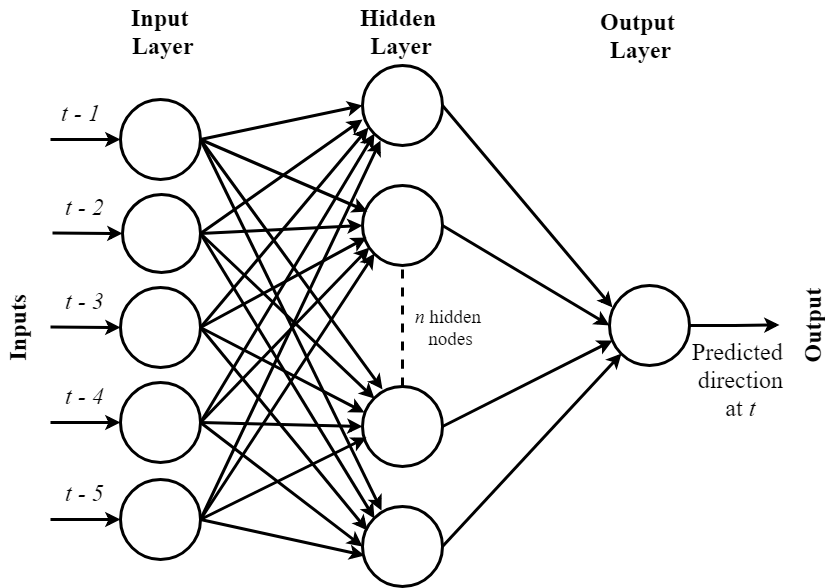
\includegraphics[width=10cm]{Base_case_diagram.png}
\centering
\caption{The feed forward architecture for the second base model.} 
\label{fig:basecase}
\end{figure}

All feed forward networks in this study followed similar network configurations. A Xavier \cite{glorot2010understanding} random initialisation was used for the initialisation of weights. The Xavier initialisation technique is designed to keep the scale of gradients approximately the same at all layers. A dropout rate of $20$\% was also applied to the input data to reduce overfitting when training. Training of data involved minimising a cross entropy cost function while using an Adam optimiser \cite{kingma2014adam}. With regards to activation function, a rectified linear unit (ReLu) was used. Since the aim of this study was not to find the state-of-the-art architecture, there was no need for an exercise to determine the best configuration for our feed forward networks, and thus it was decided to use the same configurations for all networks. 

\section{Hypothesis 1: Incorporating Other Stock Market Indices}
\label{sec:methodh1}
The architecture for this hypothesis is very similar to that used in the previous section, where a feed forward network was trained over a period of five years of data. The only different here is the number of inputs. The inputs for this architecture consisted of the closing prices from the past three days for the seven stock market indices mentioned in Table \ref{tab:indices}. Therefore, the total number of inputs for this architecture was $21$. The same exercise from the base case for finding the optimal learning rate and number of nodes was also performed. 

A closer look at the historical closing index prices of different stock markets shows that not all stock markets open on the same days. This is mainly due to stock markets not operating on country specific bank holidays. To overcome this issue, whenever an index does not have a closing price for a particular date, the last known closing price would be used instead.  

\section{Hypothesis 2: Incorporating Macroeconomic Parameters}
\label{sec:methodh2}
As per Requirement \ref{h2}, this hypothesis requires incorporating macroeconomic data with the historical closing prices of the FTSE. Section \ref{sec:discussion} mentioned the motivation for approaching this problem with an ensemble approach. 

The first stage of the ensemble consisted of training and testing several prediction models over different periods of time. The architecture for these models were similar to that used in the base case described in Section \ref{sec:thebasecase}. Models were trained and tested over periods of five years, however the period of data for each model was shifted by six months. A total of $16$ models were created, and cover stock index data from 2000 to 2013. For each model, a similar exercise to that described in Section \ref{sec:optimalparams} was performed to find the optimal parameters. Unlike in Section \ref{sec:thebasecase} and \ref{sec:methodh1}, where only the average performance was recorded for several combination of parameters, this stage only persisted the trained model that achieved the highest accuracy.  

The second stage of the ensemble involved incorporating the outputs of these pre-trained models, macroeconomic data and the closing price of the FTSE stock market index as inputs through another feed forward network, which hereafter will be referred to as the meta model. The meta model requires a different data set from the first stage for training and testing. In order to achieve a fair comparison in predictive performance, the meta model was also trained and tested with data between the year 2013 and 2018, as was done in Section \ref{sec:thebasecase} and \ref{sec:methodh1}. The optimal parameters were found using the same exercise discussed in Section \ref{sec:optimalparams}.  

Figure \ref{fig:metamodelflow} shows a high level data flow of the two-staged ensemble model. All the outputs of the pre-trained models consist of either $1$ or $0$, signifying whether they predicted the FTSE index will rise or fall. Each macroeconomic parameter consists of three inputs, which map to the actual value in the last three quarters. Finally, another three inputs were added that map to the last three closing prices of the FTSE index. 

\begin{figure}[h]
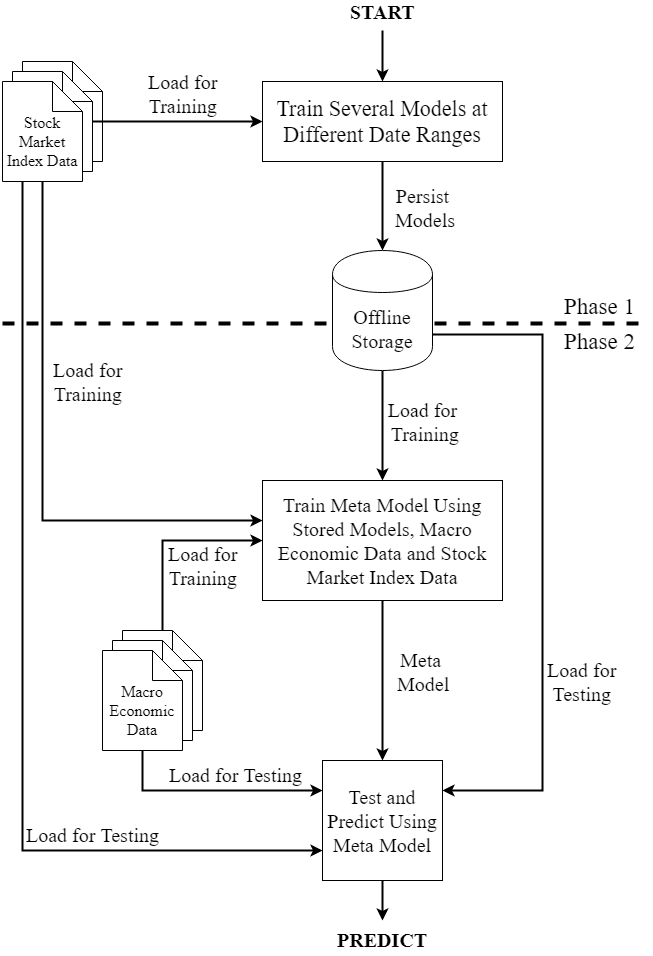
\includegraphics[width=10cm]{Meta-model.png}
\centering
\caption{The high level data flow of the two-staged ensemble model.} 
\label{fig:metamodelflow}
\end{figure}


\section{Hypothesis 3: Incorporating Macroeconomic Parameters and Other Stock Market Indices}
\label{sec:methodh3}
The exact same ensemble procedure in Section \ref{sec:methodh2} was used for this hypothesis, with the exception that each individually trained model in the first stage followed the same architecture in Section \ref{sec:methodh1} rather than the base case in Section \ref{sec:thebasecase}. 


\chapter{Results and Evaluation}
\label{cha:resultsandevaluation}
\section{The Base Cases}
All the methods mentioned in Chapter \ref{cha:implementation} were trained and tested with data from 2013 to 2018, so as to achieve a fair performance comparison over the same data set. With regards to FTSE data, this translates to $1256$ days of closing prices, therefore splitting the data $80/20$ will result in $1004$ daily closing prices for training and $252$ for testing.

\begin{figure}[h]
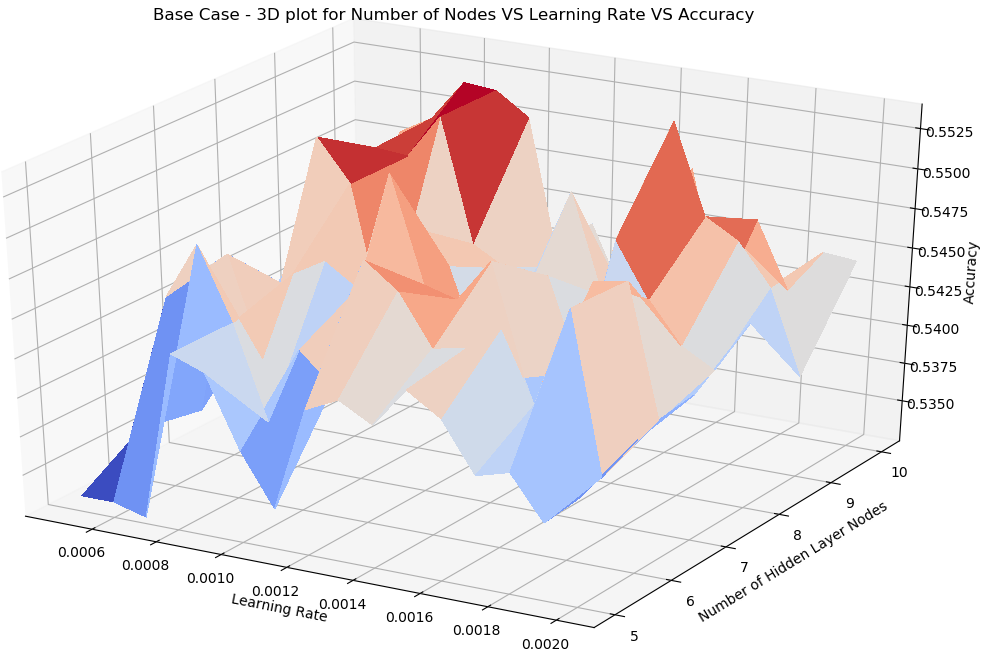
\includegraphics[width=10.5cm]{base_accuracy.png}
\centering
\caption{A 3D plot of the accuracy results for the second base case optimal parameter test.} 
\label{fig:base_plot_accuracy}
\end{figure}

With regards to the daily direction of the FTSE data, this period happens to be well balanced, where $53.18$\% of the daily FTSE closing prices rise, and $46.82$\% fall. With regards to just the testing data, the FTSE rises $51.98$\% of the time, and thus falls in the remaining $48.02$\%.

Section \ref{sec:requirements} mentions that two base cases were used. The first base case was to always predict the index as rising. Therefore, the predictive accuracy of the first base case is $51.98$\% with an F1 score of $0.684$. As mentioned in Section \ref{subsec:accuracyandf1}, since this is a well balanced data set, accuracy score will take precedence, since the F1 score is weighted more toward correctly predicting that the stock index will rise, hence the true positive.

\begin{figure}[h]
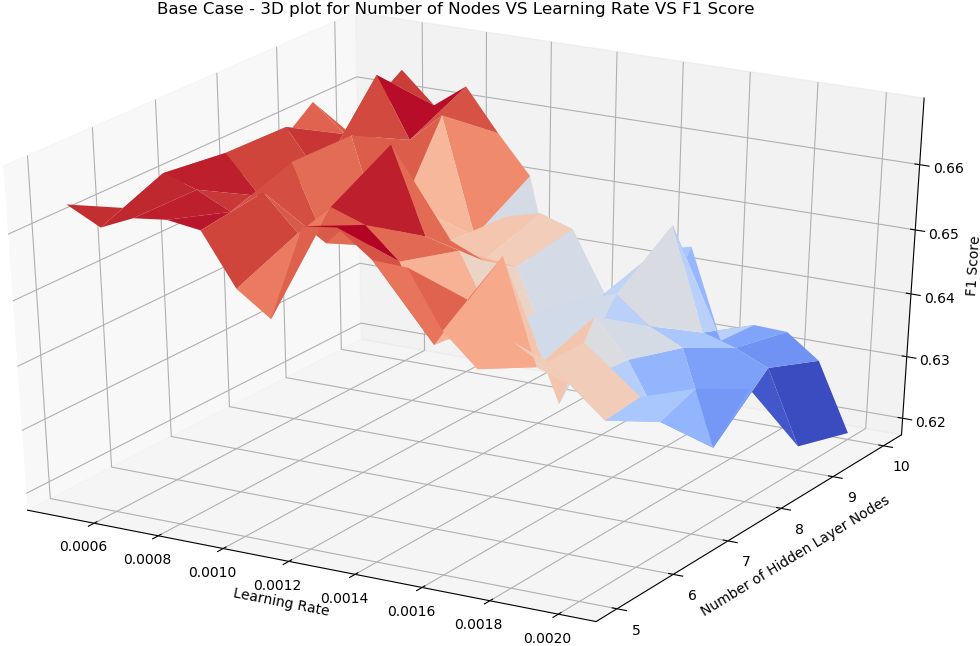
\includegraphics[width=10.5cm]{base_f1.png}
\centering
\caption{A 3D plot of the F1 score results for the second base case optimal parameter test.} 
\label{fig:base_plot_f1}
\end{figure}

The second base case consisted of implementing a simple model that predicts the direction of the FTSE index by taking as input the closing price of the index itself for the previous five days. Figure \ref{fig:base_plot_accuracy} and \ref{fig:base_plot_f1} show the results from the optimal parameter test described in Section \ref{sec:optimalparams} for the second base  case. The optimal parameters for this base case were $9$ hidden nodes with a learning rate of $0.0016$. These parameters achieved an average of $55.36$\% accuracy and $0.65$ F1 score.

Table \ref{tab:test_results} contains all the results of the experiments performed in this study. The results shows that the second base case increased accuracy with respect to the first case by $+3.37$\%, but achieved less in terms of F1 Score by $-0.0316$. The reduction in F1 score is not necessarily a bad thing for the second base case. Since the first base case predicts everything as up, then it has a perfect recall value of 1, hence resulting in a higher F1 score. 

The results of both base cases were then compared with the results of the other hypotheses.

\section{Hypothesis 1: Incorporating Other Stock Market Indices}
This hypothesis involved incorporating the closing price of other stock markets from around the world with the FTSE stock market index. Using the same data set in the previous section, Figure \ref{fig:h1_plot_accuracy} and \ref{fig:h1_plot_f1} show the results from the optimal parameter test. The best accuracy was achieved with $17$ hidden nodes and a learning rate of $0.0003$. These parameters achieved an average of $66.51$\% accuracy and an F1 score of $0.72$. Both figures produced a neat wave, where it can be shown that learning rate seems to influence the accuracy of the model more than the choice of number of hidden nodes when incorporating closing prices from other markets. 

\begin{figure}[h]
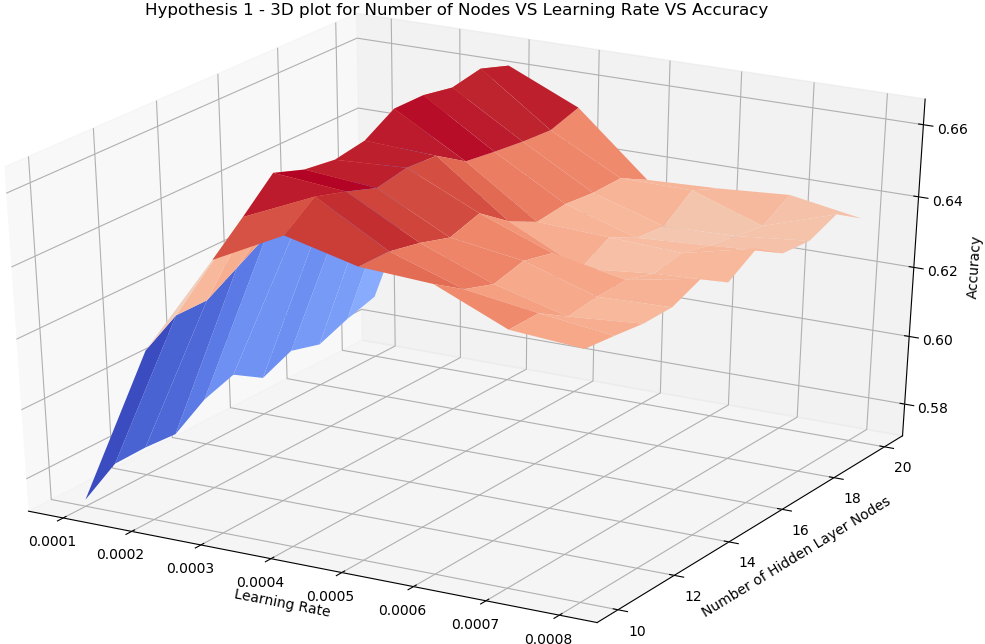
\includegraphics[width=10.5cm]{h1_accuracy.png}
\centering
\caption{A 3D plot of the accuracy results for the hypothesis \ref{h1} optimal parameter test.} 
\label{fig:h1_plot_accuracy}
\end{figure}

\begin{figure}[h]
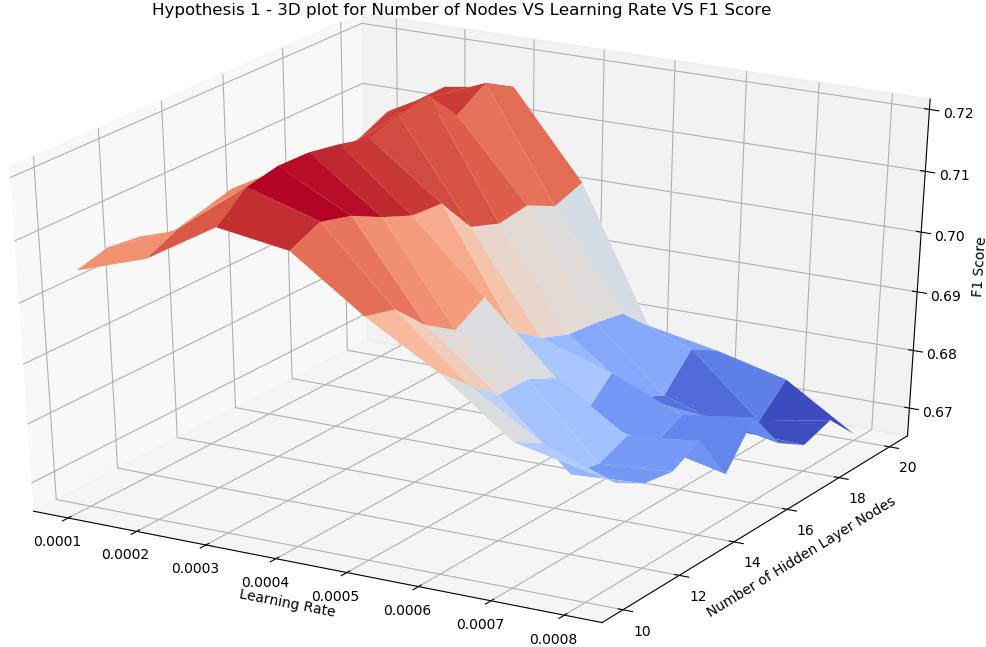
\includegraphics[width=10.5cm]{h1_f1.png}
\centering
\caption{A 3D plot of the F1 score results for the hypothesis \ref{h1} optimal parameter test.} 
\label{fig:h1_plot_f1}
\end{figure}

Taking a look at Table \ref{tab:test_results}, an increase in both accuracy and F1 score was achieved with respect to base case 1 and 2, where accuracy increased by $+14.52$\% and $+11.15$\% respectively, whereas the F1 score increased by $+0.0365$ and $+0.0681$ respectively.

\section{Hypothesis 2: Incorporating Macroeconomic Parameters}
This hypothesis involved incorporating macroeconomic parameters with the FTSE stock market index. Recall from Section \ref{sec:methodh2} that this model consists of a two staged process.

The first stage involved training models over shifted 5 year periods of data from 2000 to 2013. These models only incorporated closing prices of the FTSE index. For each period, an exercise for finding the optimal parameters was performed. Table \ref{tab:h2_stage1} shows the optimal parameters chosen for each model, which was trained and tested over a particular period, along with the accuracy and F1 score that was achieved. 
\begin{table}[h]
    \centering
    \begin{tabular}{|c|c|c|c|c|} \hline
        \textbf{Model Period} & \textbf{Learning Rate} & \textbf{Nodes} & \textbf{F1 Score} & \textbf{Accuracy} \\ \hline
        Jan 2000 - 2005 & 0.0013 & 16 & 0.489 & 0.516 \\
        Jul 2000 - 2005 & 0.0005 & 14 & 0.548 & 0.532 \\
        Jan 2001 - 2006 & 0.0011 & 18 & 0.634 & 0.552 \\
        Jul 2001 - 2006 & 0.0011 & 10 & 0.663 & 0.562 \\
        Jan 2002 - 2007 & 0.0009 & 12 & 0.631 & 0.510 \\
        Jul 2002 - 2007 & 0.0005 & 07 & 0.691 & 0.562 \\
        Jan 2003 - 2008 & 0.0005 & 08 & 0.652 & 0.558 \\
        Jul 2003 - 2008 & 0.0009 & 09 & 0.594 & 0.556 \\
        Jan 2004 - 2009 & 0.0011 & 18 & 0.534 & 0.488 \\
        Jul 2004 - 2009 & 0.0011 & 10 & 0.555 & 0.516 \\
        Jan 2005 - 2010 & 0.0007 & 09 & 0.642 & 0.579 \\
        Jul 2005 - 2010 & 0.0011 & 07 & 0.584 & 0.536 \\
        Jan 2006 - 2011 & 0.0013 & 18 & 0.653 & 0.583 \\
        Jul 2006 - 2011 & 0.0011 & 20 & 0.620 & 0.552 \\
        Jan 2007 - 2012 & 0.0005 & 12 & 0.587 & 0.508 \\
        Jul 2007 - 2012 & 0.0011 & 20 & 0.546 & 0.532 \\
        \hline
    \end{tabular}
    \caption{The chosen parameters and performance results for each model trained over its respective period in the first stage of the ensemble for Hypothesis \ref{h2}.}
    \label{tab:h2_stage1}
\end{table}

\begin{figure}[h]
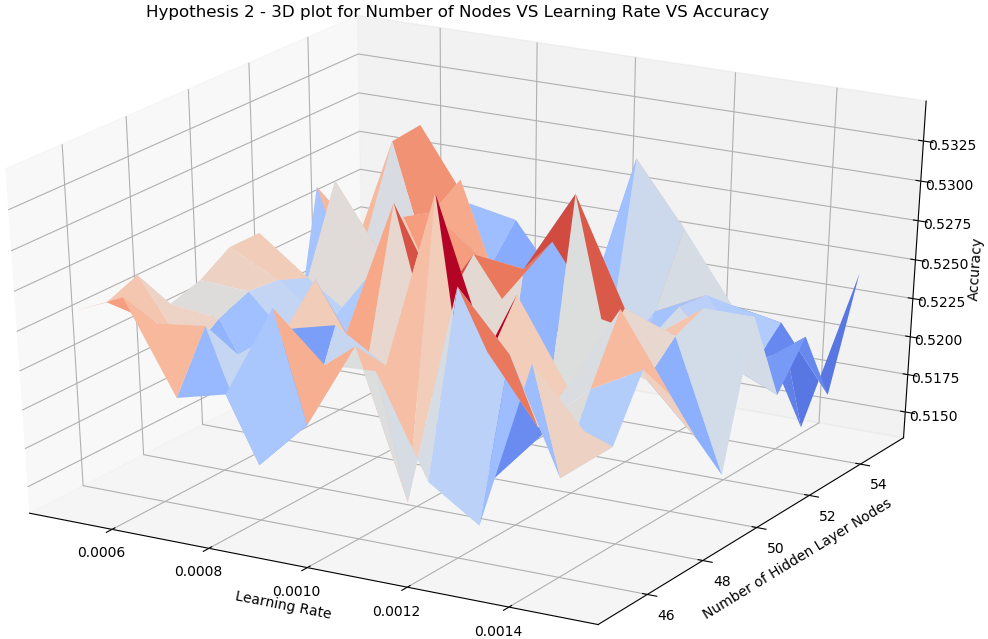
\includegraphics[width=10.5cm]{h2_accuracy.png}
\centering
\caption{A 3D plot of the accuracy results for the hypothesis \ref{h2} optimal parameter test.} 
\label{fig:h2_plot_accuracy}
\end{figure}

\begin{figure}[h]
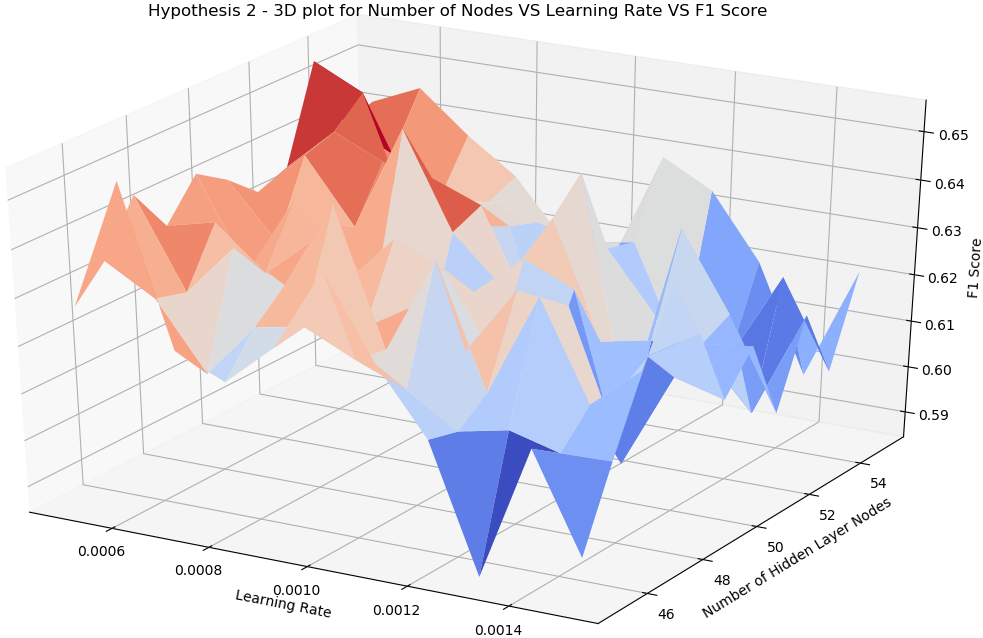
\includegraphics[width=10.5cm]{h2_f1.png}
\centering
\caption{A 3D plot of the F1 score results for the hypothesis \ref{h2} optimal parameter test.} 
\label{fig:h2_plot_f1}
\end{figure}

The second stage involved incorporating the predictions form these models with lagged macroeconomic data. Figure \ref{fig:h2_plot_accuracy} and \ref{fig:h2_plot_f1} show the results from the optimal parameter test for the second stage. The best accuracy was achieved with learning rate $0.0011$ and $47$ hidden nodes. 
As shown in Table \ref{tab:test_results}, disappointing results were achieved. This hypothesis did not perform better than the second base case in terms of both accuracy and F1 score, and only achieved a small increase in accuracy over the first base case. With respect to accuracy, this hypothesis achieved $+1.47$\% and $-0.0191$\% compared to base case 1 and 2, and  $-0.0425$ and $-0.0109$ for the F1 score.   

\section{Hypothesis 3: Incorporating Macroeconomic Parameters and Other Stock Market Indices}
This hypothesis followed a similar approach to that in the previous hypothesis, with the exception that each model trained in the first stage also incorporated closing prices from other stock markets. Table \ref{tab:h3_stage1} shows the optimal parameters chosen for each period in the first stage of the process, along with the achieved accuracy and F1 score. 


\begin{table}[h]
    \centering
    \begin{tabular}{|c|c|c|c|c|} \hline
        \textbf{Data Period} & \textbf{Learning Rate} & \textbf{Nodes} & \textbf{F1 Score} & \textbf{Accuracy} \\ \hline
        Jan 2000 - 2005 & 0.0008 & 12 & 0.669 & 0.640\\
        Jul 2000 - 2005 & 0.0004 & 14 & 0.681 & 0.652\\
        Jan 2001 - 2006 & 0.0009 & 16 & 0.695 & 0.632\\
        Jul 2001 - 2006 & 0.0017 & 19 & 0.688 & 0.614\\
        Jan 2002 - 2007 & 0.0007 & 17 & 0.648 & 0.602\\
        Jul 2002 - 2007 & 0.0013 & 15 & 0.655 & 0.610\\
        Jan 2003 - 2008 & 0.0001 & 23 & 0.703 & 0.653\\
        Jul 2003 - 2008 & 0.0003 & 19 & 0.715 & 0.706\\
        Jan 2004 - 2009 & 0.0003 & 25 & 0.653 & 0.671\\
        Jul 2004 - 2009 & 0.0002 & 12 & 0.694 & 0.671\\
        Jan 2005 - 2010 & 0.0003 & 15 & 0.715 & 0.687\\
        Jul 2005 - 2010 & 0.0005 & 17 & 0.704 & 0.667\\
        Jan 2006 - 2011 & 0.0005 & 19 & 0.671 & 0.627\\
        Jul 2006 - 2011 & 0.0001 & 17 & 0.703 & 0.671\\
        Jan 2007 - 2012 & 0.0009 & 21 & 0.649 & 0.623\\
        Jul 2007 - 2012 & 0.0015 & 23 & 0.643 & 0.603\\
        \hline
    \end{tabular}
    \caption{The chosen parameters and performance results for each model trained over its respective period in the first stage of the ensemble for Hypothesis \ref{h3}.}
    \label{tab:h3_stage1}
\end{table}

Regarding the second stage, Figure \ref{fig:h3_plot_accuracy} and \ref{fig:h3_plot_f1} show the results from the optimal parameter test. The best accuracy was achieved with a learning rate of $0.00001$ and $56$ hidden nodes. Similar to hypothesis 1, this hypothesis achieved a higher accuracy and F1 score compared to both base cases. Accuracy increased by $+1.15$\% and $+8.12$\% compared to the first and second base case, while the F1 score increased by $+0.0237$ and $+0.0553$ respectively.

\begin{figure}[h]
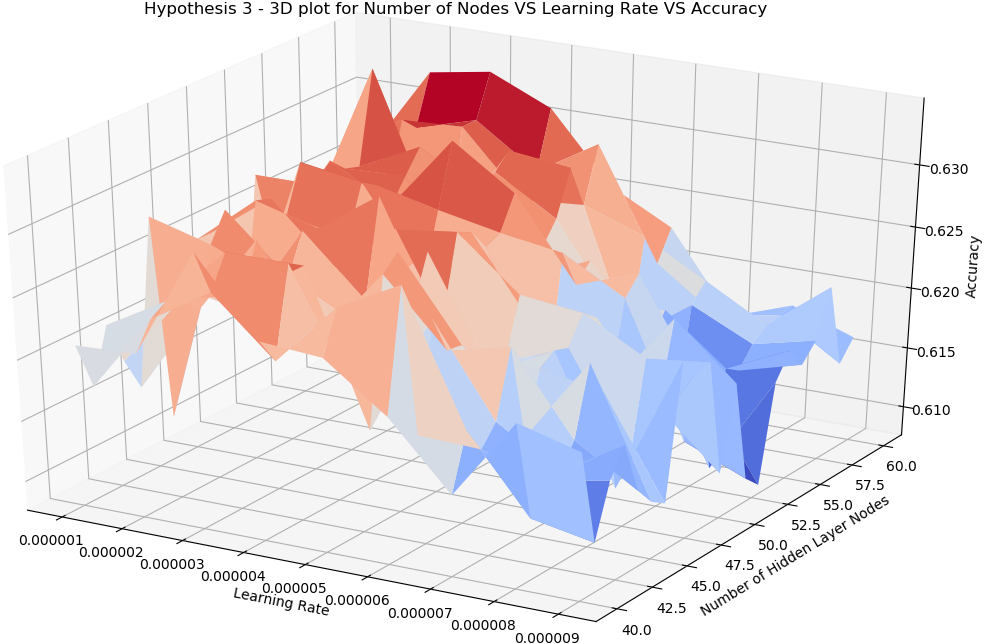
\includegraphics[width=10.5cm]{h3_accuracy.png}
\centering
\caption{A 3D plot of the accuracy results for the hypothesis \ref{h3} optimal parameter test.} 
\label{fig:h3_plot_accuracy}
\end{figure}

\begin{figure}[h]
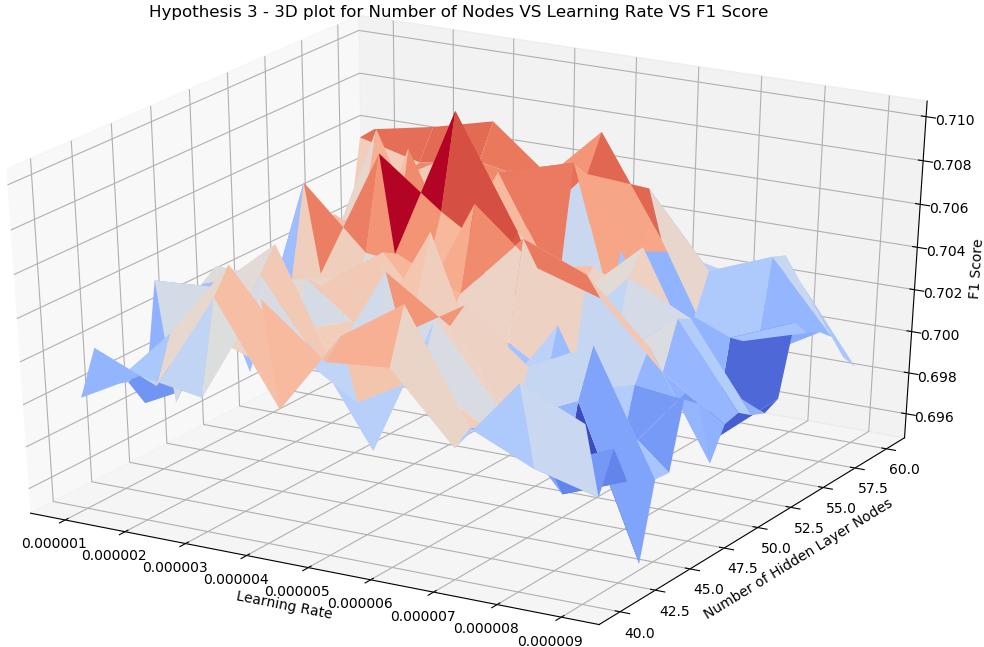
\includegraphics[width=10.5cm]{h3_f1.png}
\centering
\caption{A 3D plot of the F1 score results for the hypothesis \ref{h3} optimal parameter test.} 
\label{fig:h3_plot_f1}
\end{figure}

\begin{table}[h]
    \centering
    \begin{tabular}{|c|c|c|c|c|} \hline
        \textbf{Method} & \textbf{Learning Rate} & \textbf{Nodes} & \textbf{Accuracy} & \textbf{F1 Score} \\ \hline
        \textbf{Base Case 1} & - & - & 0.51984 & 0.68404 \\
        \textbf{Base Case 2} & 0.0016 & 09 & 0.55357 & 0.65241 \\
        \textbf{Hypothesis \ref{h1}} & 0.0003 & 17 & 0.66508 & 0.72052 \\
        \textbf{Hypothesis \ref{h2}} & 0.0011 & 47 & 0.53452 & 0.64150 \\
        \textbf{Hypothesis \ref{h3}} & 0.00001 & 56 & 0.63472 & 0.70772  \\
        \hline
    \end{tabular}
    \caption{Table of optimal parameters and maximising the average performance metrics for each method.}
    \label{tab:test_results}
\end{table}



\section{Statistical Significance Tests}
Section \ref{sec:statisticalsignificancetest} explained how the Kruskal-Wallis and Wicoxon signed rank tests can be used to determine whether any significant increase in accuracy is achieved between different methods. 

The first step was to perform the Kruskal-Wallis test on all the prediction outputs of each method simultaneously, which are the two base cases and hypothesis \ref{h1}, \ref{h2} and \ref{h3}. The p-value given by this test was of \textbf{$0.0006316$}. Since this is less than $0.05$, the null-hypothesis is rejected, therefore at least one sample does not originate from the same population, ergo has a significant difference in accuracy.

The next step was to perform the Wilcoxon signed rank test on all pairs of results. Table \ref{tab:wilcoxon_results} consists of a matrix of the resulting p-values from the test for each given pair. The values that are in bold are greater than 0.005, thus the null hypothesis had been accepted for that given pair. This means that no significant improvement in accuracy was achieved from:
\begin{enumerate}
    \item The second base case with respect to the first base case.
    \item The second hypothesis with respect to the second base case.
    \item The third hypothesis with respect to the first hypothesis.
\end{enumerate}

The null hypothesis for each hypothesis in Section \ref{sec:objectives} was defined as the method in question not achieving a significant difference in accuracy when compared to  underlying base cases. This means that the null hypothesis for hypothesis \ref{h2} can be accepted, while the null hypothesis for both hypothesis \ref{h1} and \ref{h3} can be rejected.

\begin{table}[h]
    \centering
    \begin{tabular}{|c|c|c|c|c|c|} \hline
         &  \textbf{BC 1} & \textbf{BC 2} & \textbf{H1} & \textbf{H2} & \textbf{H3} \\ \hline
        \textbf{BC1} & - & \textbf{0.07044} & 0.00000459 &  0.01431 & 0.0000712\\
        \textbf{BC2} & \textbf{0.07044} & - & 0.00176 & \textbf{1.0} & 0.02771 \\
        \textbf{H1} & 0.00000459 & 0.00176 & - & 0.001216 & \textbf{0.15985} \\
        \textbf{H2} & 0.01431 & \textbf{1.0} & 0.001216 & - & 0.01532\\
        \textbf{H3} & 0.0000712 & 0.02771 & \textbf{0.15985} & 0.01532 & -  \\
        \hline
    \end{tabular}
    \caption{Matrix of p-values for performing the Wilcoxon signed rank test on pairs of results. P-values that are in bold mean that the hypothesis has been accepted, therefore there is no significant difference in accuracy between the pair. }
    \label{tab:wilcoxon_results}
\end{table}


\chapter{Conclusion and Future Work}
\label{cha:conclusions}

\section{Summary}
Stock market prediction provides an excellent opportunity for entities such as investment firms to maximise on profits by making informed decisions on whether to buy or hold stock based on the market predicted outcome. This is no trivial task however, as stock markets are chaotic in nature and continuously fluctuating. Literature has shown that choosing the right data is crucial when it comes to financial forecasting. This study sought to measure the impact that macroeconomic data and closing prices from global markets have on predicting the direction of the FTSE stock market index. 

Three hypotheses were formulated with the aim of determining whether any significant improvement in accuracy is achieved when comparing with underlying base cases. The base cases involved two models, one that always predicted the direction of the FTSE index as up, and the other a simple model that only uses FTSE closing data from the past few days. Three other experiments that represent the three hypotheses involved creating:
\begin{enumerate}
    \item a model that incorporated closing prices from other stock markets with FTSE data.
    \item a model that incorporated macroeconomic parameters with FTSE data.
    \item a model that incorporated both macroeconomic parameters and closing prices from other stock markets with FTSE data. 
\end{enumerate}

An exercise had to be performed for finding the optimal learning rate and number of hidden nodes for each feed forward network in the study. Predictive performance was measured using the accuracy and F1 score metrics, while the Kruskal-Wallis and Wicoxon signed rank tests were used to determine whether any significant increase in accuracy was achieved when compared with the base cases. The following section discusses the findings of this study.

\section{Discussion}
 The worst performing model was hypothesis \ref{h2} which did not achieve a significant improvement in accuracy over the second base case. Hypothesis \ref{h3}, which just like hypothesis \ref{h2} incorporates macroeconomic parameters, also did not achieve any significant increase in accuracy over hypothesis \ref{h1}. These two observations seem to suggest that incorporating macroeconomic parameters into models does not help increase predictive performance. This may be true, however there could be an alternative reason to these results. While the macroeconomic parameters chosen are regarded as important parameters for describing the state of an economy, the possibility remains that these parameters were not the most suitable macroeconomic parameters to stock market prediction. This study, given more time, could have performed a more informed exercise for determining the macroeconomic parameters with the highest correlation with stock market indices. Another possibility is that the chosen ensemble approach with two feed forward network stages was not ideal for incorporating such data. There is also the possibility that the way the macroeconomic parameters were preprocessed and fed into the meta model as lagged quarterly data was not ideal. Clearly, there is plenty of room for improvement with regards to incorporating macroeconomic data. 

On the other hand, incorporating closing stock prices from global markets was a success, with hypothesis \ref{h1} achieving the best accuracy. Interestingly, the ensemble approach in hypothesis \ref{h3} did not outperform the single staged feed forward model, which suggests that less complex architectures do perform best. This also supports the earlier argument about the chosen ensemble approach not being suitable for incorporating macroeconomic data in such a way. While the chosen ensemble approach may not have been the ideal choice of architecture, given more time, it would have been interesting to compare hypothesis \ref{h1} with a similar ensemble that naively only takes the most common prediction from the pre-trained models.

While this study showed that external data does help improve the prediction accuracy of model, it also showed that it is not always obvious which data is best, and thus a lot more effort must be made into finding the most influential data for improving a model.

\section{Future Work}
Time was a limiting factor in this study. Had this not been the case, the following could have been attempted:
\begin{itemize}
    \item \textbf{Experiment with other architectures, other than feed forward networks.} This study skimmed over different approaches such as using genetic algorithms, recurrent neural networks, SVM and deep learning. Feed forward networks were chosen because they are non complex yet still effective, and because the main aim was not to find the state-of-the art approach, but to measure impact of using certain data. Nonetheless, another architecture could have be more suitable for incorporating macroeconomic data. 
    \item \textbf{Perform an exercise to find suitable macroeconomic parameters.} The five macroeconomic parameters used in this study were chosen because they are considered important parameters for describing an economy. Clearly, better parameters could have been chosen. The reason for choosing only five was to keep things simple. 
    \item \textbf{Predict the actual closing price or percentage increase of the FTSE index}. It was decided to stick to predicting the direction not only for simplicity, but also because the study was only interested in the impact of data, rather than to try and measure profits. Financial forecasting as a regression problem rather than a binary problem is more useful in the real world. Predicting whether a stock will rise or fall would not equate to profit, because a single wrong prediction could easily be large enough to wipe out any profits made in the past. A more ambitious idea would be to incorporate this study into a trading strategy and measure the impact of data on increasing profits. 
\end{itemize}

\printbibliography
\end{document}